\documentclass[11pt,a4paper,twoside]{report}

\usepackage[dvipsnames,table,xcdraw]{xcolor}
\usepackage[all]{xy}
\usepackage[brazilian]{babel}
\usepackage[utf8]{inputenc}

\usepackage[T1]{fontenc}
\usepackage[sfdefault,scaled=.85]{FiraSans}
\usepackage{newtxsf}
\let\openbox\relax

\usepackage{framed}
\usepackage{cancel}
\usepackage{xfrac}
\usepackage{enumerate} 
\usepackage{enumitem}
\usepackage{amssymb}
\usepackage{amsmath}
\usepackage{amsthm}
\usepackage{amscd}
\usepackage{amsfonts}
\usepackage{mathrsfs}
\usepackage{mathtools}
\usepackage{bm}
\usepackage{tikz-cd}
\usepackage{tikz}
\usepackage{forest}
\usepackage[skip=1pt,font=footnotesize]{caption}
\usepackage{subcaption}
\usepackage{float}
\usetikzlibrary{shadows,shapes.geometric}
\usetikzlibrary{calc}
\usepackage{enumerate}
\usepackage[pdftex]{hyperref}
 \hypersetup{
     colorlinks=true,
     linkcolor=chromeyellow,
     filecolor=chromeyellow,
     citecolor = chromeyellow,      
     urlcolor=chromeyellow,
     }
\usepackage[most,breakable]{tcolorbox}
\usepackage{titletoc}
\usepackage{sidecap}
\usepackage[sort,authoryear]{natbib}
\usepackage{import}

\usepackage{appendix}
\usepackage{moresize}
\usepackage{anyfontsize}
\usepackage{titlesec}
\usepackage{epigraph}
\usepackage{booktabs}
\usepackage{multirow}
\usepackage{rotating}
\usepackage{varwidth}

\usepackage[a4paper,top=3cm,bottom=2cm,left=3cm,right=2cm]{geometry}

\usepackage{wrapfig}
\usepackage{indentfirst}

%\definecolor{lightgray}{gray}{0.95}
\usepackage{minted}
\usemintedstyle{vs}%{vs}%{pastie}%{autumn}%{emacs}%{tango}%{rrt}%{manni}
\setminted{
	fontsize=\footnotesize, 
	breaklines=true, 
	breakafter={.,\space}, 
	breakbytokenanywhere=true, 
	numbers=left, 
	frame=lines,
	framerule=0.5pt,
	rulecolor=\color{chromeyellow!30},
	numbersep=5pt, 
	bgcolor=white,
	baselinestretch = 1,
	linenos=false
}


% Fixando as fontes
\DeclareFixedFont{\ttm}{T1}{txtt}{m}{n}{8}  % normal

% Estilo para Código de Output
\newcommand\pythonoutputstyle{\lstset{
		basicstyle=\ttm\color{chromeyellow}, % Estilo para o output
		breaklines=true,
		literate=
		{á}{{\'a}}1
		{à}{{\`a}}1
		{ã}{{\~a}}1
		{é}{{\'e}}1
		{ê}{{\^e}}1
		{í}{{\'i}}1
		{ó}{{\'o}}1
		{õ}{{\~o}}1
		{ú}{{\'u}}1
		{ü}{{\"u}}1
		{ç}{{\c{c}}}1
		{ü}{{\"u}}1
		{ŋ}{{\ng}}1
}}

% Ambiente para Código de Output
\lstnewenvironment{pythonoutput}[1][]
{
	\pythonoutputstyle
	\lstset{#1}
}
{}

\sloppy
\interfootnotelinepenalty=10000
\allowdisplaybreaks
\raggedbottom

%%%%%%%%%%%%

\makeatletter
\titleformat{\part}[display]
{\Huge\scshape\filright\color{white}}
{\partname~\thepart:}
{0pt}
{\colorbox{chromeyellow}}
\makeatother

%%%%%%%%%%%%%%%%%%%%%%%%%%%

\definecolor{chromeyellow}{rgb}{0.03, 0.15, 0.4}

\usepackage{fancyhdr}
\fancyhead{}
\fancyfoot{}
\colorlet{myfancycolor}{chromeyellow!60!white}
\makeatletter
\def\headrule{\color{myfancycolor}{\if@fancyplain\let\headrulewidth\plainheadrulewidth\fi
		\hrule\@height\headrulewidth\@width\headwidth
		\vskip-\headrulewidth}}
\makeatother

\fancypagestyle{mystyle}{
	\renewcommand*\headrulewidth{2pt}
	\fancyfoot[OR]{%
		\color{myfancycolor}%
		\rule[-6pt]{100pt}{20pt}%
		\hspace*{-90pt}%
		\begin{minipage}[b]{0.5cm}%
			\color{white}%
			\textsf{\thepage}%
		\end{minipage}%
	}%
	\fancyfoot[EL]{%
		\hspace*{-75pt}%
		\color{myfancycolor}%
		\rule[-6pt]{100pt}{20pt}%
		\hspace*{-25pt}%
		\begin{minipage}[b]{0.5cm}%
			\color{white}%
			\hfill%
			\textsf{\thepage}%
		\end{minipage}%
	}%
	\fancyhead[OR]{%
		\raisebox{0.5em}{\sffamily\nouppercase{\rightmark}}\space\color{myfancycolor}\rule{2em}{2em}\raisebox{0.5em}{\hspace{-2em}\color{white}\makebox[2em][c]{\textsf{\thechapter}}}%
		\vspace*{-0.5em}%
	}
	\fancyhead[EL]{%
		\color{myfancycolor}\rule{2em}{2em}\raisebox{0.5em}{\hspace{-2em}\color{white}\makebox[2em][c]{\textsf{\thechapter}}}\color{black}\raisebox{0.5em}{\space\sffamily\nouppercase{\rightmark}}%
		\vspace*{-0.5em}%
	}   
}

\fancypagestyle{plain}{%
	\renewcommand*\headrulewidth{0pt}
	\fancyhf{}%
	\fancyfoot[OR]{%
		\color{myfancycolor}%
		\rule[-6pt]{100pt}{20pt}%
		\hspace*{-90pt}%
		\begin{minipage}[b]{0.5cm}%
			\color{white}%
			\textsf{\thepage}%
		\end{minipage}%
	}%
	\fancyfoot[EL]{%
		\hspace*{-75pt}%
		\color{myfancycolor}%
		\rule[-6pt]{100pt}{20pt}%
		\hspace*{-25pt}%
		\begin{minipage}[b]{0.5cm}%
			\color{white}%
			\hfill%
			\textsf{\thepage}%
		\end{minipage}%
	}%
}   
\fancypagestyle{unnumbered}{%
	\fancyhead[OR]{%
		\raisebox{0.5em}{\sffamily\nouppercase{\rightmark}}\space\color{myfancycolor}\rule{2em}{2em}%
		\vspace*{-0.5em}%
	}
	\fancyhead[EL]{%
		\color{myfancycolor}\rule{2em}{2em}\color{black}\raisebox{0.5em}{\space\sffamily\nouppercase{\rightmark}}%
		\vspace*{-0.5em}%
	}
}

\pagestyle{mystyle}
\renewcommand{\chaptermark}[1]{\markboth{#1}{#1}}
\renewcommand*{\sectionmark}[1]{} %
\theoremstyle{plain}
\newtcbtheorem[auto counter, number within=chapter]{exemplo}{\strut Exemplo}{
    enhanced jigsaw,
    breakable,
    sharp corners,
    boxrule=0pt,
    toprule=1pt,bottomrule=1pt,
    left=0.2cm,right=0.2cm,top=0.2cm,
    colframe=chromeyellow!75,
    colback=white,
    colbacktitle=chromeyellow!75,
    coltitle=white,
    before skip=15pt plus 2pt,
    after skip=15pt plus 2pt 
}{th}

\newtcbtheorem[number within=chapter]{teo}{\strut Teorema}{
    enhanced,
    colframe=chromeyellow!75,
    colback=white,
    colbacktitle=chromeyellow!75,
    coltitle=white,
    boxed title style={},
    attach boxed title to top left={xshift=5mm,yshift*=-\tcboxedtitleheight/2},
    before skip=25pt plus 2pt,
    after skip=15pt plus 2pt
}{th}

\newtcbtheorem[number within=chapter]{df}{\strut Definição}{
    enhanced,
    colframe=chromeyellow!75,
    colback=white,
    colbacktitle=chromeyellow!75,
    coltitle=white,
    boxed title style={},
    attach boxed title to top left={xshift=5mm,yshift*=-\tcboxedtitleheight/2},
    before skip=25pt plus 2pt,
    after skip=15pt plus 2pt
}{th}

\newtcbtheorem[number within=chapter]{prop}{\strut Proposição}{
    enhanced,
    colframe=chromeyellow!75,
    colback=white,
    colbacktitle=chromeyellow!75,
    coltitle=white,
    boxed title style={},
    attach boxed title to top left={xshift=5mm,yshift*=-\tcboxedtitleheight/2},
    before skip=25pt plus 2pt,
    after skip=15pt plus 2pt
}{th}

\newtcbtheorem[number within=chapter]{coro}{\strut Corolário}{
    enhanced,
    colframe=chromeyellow!75,
    colback=white,
    colbacktitle=chromeyellow!75,
    coltitle=white,
    boxed title style={},
    attach boxed title to top left={xshift=5mm,yshift*=-\tcboxedtitleheight/2},
    before skip=25pt plus 2pt,
    after skip=15pt plus 2pt
}{th}

\newtcbtheorem[number within=chapter]{lema}{\strut Lema}{
    enhanced,
    colframe=chromeyellow!75,
    colback=white,
    colbacktitle=chromeyellow!75,
    coltitle=white,
    boxed title style={},
    attach boxed title to top left={xshift=5mm,yshift*=-\tcboxedtitleheight/2},
    before skip=25pt plus 2pt,
    after skip=15pt plus 2pt
}{th}

\theoremstyle{definition}
\newtheorem{ex}{Exemplo}

\newtheorem{problema}{Problema}
\makeatletter
\@addtoreset{problema}{section}
\makeatother

\definecolor{light-gray}{gray}{0.95}
\newcommand{\code}[1]{\colorbox{light-gray}{\small{\texttt{#1}}}}
\titleformat{\chapter}[block]%
        {\normalfont\scshape\HUGE}%
        {\hspace*{0pt}\color{chromeyellow!75}\fontencoding{U}\fontfamily{eur}\fontseries{b}\fontsize{60}{80}\selectfont\thechapter\hspace{15pt}}{10pt}
        {}[\chapterdecoration]

\newcommand\chapterdecoration{%
\begin{tikzpicture}[remember picture,overlay,shorten >= -10pt]

\coordinate (aux1) at ([yshift=-15pt]current page.north east);
\coordinate (aux2) at ([yshift=-410pt]current page.north east);
\coordinate (aux3) at ([xshift=-4.5cm]current page.north east);
\coordinate (aux4) at ([yshift=-150pt]current page.north east);

\begin{scope}[chromeyellow!20,line width=12pt,rounded corners=12pt]
\draw
  (aux1) -- coordinate (a)
  ++(225:5) --
  ++(-45:5.1) coordinate (b);
\draw[shorten <= -10pt]
  (aux3) --
  (a) --
  (aux1);
\draw[opacity=0.6,chromeyellow,shorten <= -10pt]
  (b) --
  ++(225:2.2) --
  ++(-45:2.2);
\end{scope}
\draw[chromeyellow,line width=8pt,rounded corners=8pt,shorten <= -10pt]
  (aux4) --
  ++(225:0.8) --
  ++(-45:0.8);
\begin{scope}[chromeyellow!30,line width=6pt,rounded corners=8pt]
\draw[shorten <= -10pt]
  (aux2) --
  ++(225:3) coordinate[pos=0.45] (c) --
  ++(-45:3.1);
\draw
  (aux2) --
  (c) --
  ++(135:2.5) --
  ++(45:2.5) --
  ++(-45:2.5) coordinate[pos=0.3] (d);   
\draw 
  (d) -- +(45:1);
\end{scope}
\end{tikzpicture}%
}


\everymath{\displaystyle}

%\setlength{\parindent}{1.5em}
%\renewcommand{\baselinestretch}{1.5}

% não permite separação silábica
%\sloppy
%\hyphenpenalty=100000
% não permite linhas orfãs e viúvas no tex
\clubpenalty=10000
\widowpenalty=10000
\displaywidowpenalty=10000
\definecolor{chromeyellow}{rgb}{0.03, 0.15, 0.4}
	
\newcommand{\tituloum}[5]{\begin{titlepage} 
    \pagecolor{chromeyellow}
    \color{white}
	\centering 
	
	\scshape 
	
	\vspace*{\baselineskip}

	
	\rule{\textwidth}{1.6pt}\vspace*{-\baselineskip}\vspace*{2pt} 
	\rule{\textwidth}{0.4pt} 
	
	\vspace{0.75\baselineskip} 
	
	{\LARGE #1} 
	
	\vspace{0.75\baselineskip}
	
	\rule{\textwidth}{0.4pt}\vspace*{-\baselineskip}\vspace{3.2pt}
	\rule{\textwidth}{1.6pt}
	
	\vspace{2\baselineskip}
	
	#2
	
	\vspace*{3\baselineskip}
	
	Autor
	
	\vspace{0.5\baselineskip}
	
	{\scshape\Large #3}
	
	\vspace{0.5\baselineskip}
	
	\textit{#4}
	
	\vfill
	
	\vspace{0.3\baselineskip}
	
	#5

\end{titlepage}
\nopagecolor}
\titlecontents{chapter}[1.5pc]
{\addvspace{30pt}}%
{\begin{tikzpicture}[remember picture, overlay]%
		\draw[fill=chromeyellow!80,draw=chromeyellow!80] (-4,-.3) rectangle (-0.3,.6);%
		\pgftext[left,x=-1cm,y=0.2cm]{\color{white}\Large\sc\bfseries                         
			\thecontentslabel};%
	\end{tikzpicture}\color{chromeyellow!90}\large\sc\bfseries}
{\color{chromeyellow!90}\large\sc\bfseries}
{\color{chromeyellow!90}\;\titlerule \;\large\sc\bfseries \thecontentspage
	\begin{tikzpicture}[remember picture, overlay]
		\draw[fill=chromeyellow!70,draw=chromeyellow!70] (2pt,0) rectangle (6,0.1pt);
\end{tikzpicture}}%

\titlecontents{section}[3.8pc]
{\addvspace{3pt}}
{\contentslabel[\thecontentslabel]{2.4pc}}
{}
{\dotfill\small \thecontentspage}
[]
\titlecontents{subsection}[5pc]
{\addvspace{1pt}}
{\contentslabel[\thecontentslabel]{2.4pc}}
{}
{\dotfill\small \thecontentspage}
[]
\makeatletter

\renewcommand{\tableofcontents}{%
	\chapter*{%
		\vspace*{-20\p@}%
		\begin{tikzpicture}[remember picture, overlay]%
			\pgftext[right,x=14.84cm,y=0.2cm]{\color{chromeyellow!80}\Huge\sc\bfseries    
				\contentsname};%
			\draw[fill=chromeyellow!80,draw=chromeyellow!80] (13,-.75) rectangle (20,1);%
			\clip (13,-.75) rectangle (20,1);
			\pgftext[right,x=14.84cm,y=0.2cm]{\color{white}\Huge\sc\bfseries 
				\contentsname};%
	\end{tikzpicture}}%
	\@starttoc{toc}}
\makeatother
\everymath{\displaystyle}

\begin{document}

\begin{titlepage}
\pagestyle{empty}

% Background color
\begin{tikzpicture}[remember picture,overlay]
\fill[chromeyellow] (current page.south west) rectangle (current page.north east);


% Background Hexagon
\begin{scope}
\foreach \i in {2.5,...,22}
{\node[rounded corners,chromeyellow!90,draw,regular polygon,regular polygon sides=6, minimum size=\i cm,ultra thick] at ($(current page.west)+(2.5,-5)$) {} ;}
\end{scope}

\foreach \i in {0.5,...,22}
{\node[rounded corners,chromeyellow!90,draw,regular polygon,regular polygon sides=6, minimum size=\i cm,ultra thick] at ($(current page.north west)+(2.5,0)$) {} ;}

\foreach \i in {0.5,...,22}
{\node[rounded corners,chromeyellow!98,draw,regular polygon,regular polygon sides=6, minimum size=\i cm,ultra thick] at ($(current page.north east)+(0,-9.5)$) {} ;}

\foreach \i in {21,...,6}
{\node[chromeyellow!95,rounded corners,draw,regular polygon,regular polygon sides=6, minimum size=\i cm,ultra thick] at ($(current page.south east)+(-0.2,-0.45)$) {} ;}

% Title of the Report
\node[left,chromeyellow!10,minimum width=0.625*\paperwidth,minimum height=3cm, rounded corners] at ($(current page.north east)+(0,-9.5)$){{\fontsize{20}{25} \selectfont \bfseries ESTATÍSTICA E}};

\node[left,chromeyellow!10,minimum width=0.625*\paperwidth,minimum height=3cm, rounded corners] at ($(current page.north east)+(0,-10.5)$){{\fontsize{20}{25} \selectfont \bfseries ANÁLISE DE DADOS CIENTÍFICOS}};

% Author Name
\node[left,chromeyellow!5,minimum width=0.625*\paperwidth,minimum height=2cm, rounded corners] at ($(current page.north east)+(0,-12)$){{\textsc{Sarah G. A. Barbosa}}};

% Year
\node[rounded corners,fill=chromeyellow!95,text =BlueViolet!5,regular polygon,regular polygon sides=6, minimum size=2.5 cm,inner sep=0,ultra thick] at ($(current page.west)+(2.5,-5)$) {\LARGE \bfseries 2024};
\end{tikzpicture}
\end{titlepage}

\thispagestyle{empty}
\pagenumbering{roman}
\tableofcontents

\newpage

\pagenumbering{arabic}

\pagecolor{chromeyellow}

\part{Probabilidade, variáveis aleatórias e estatísticas}

\pagecolor{white}

\chapter{Teoria da Probabilidade}\label{cap:1-1}

\section{Experimentos e Eventos}

Todo experimento tem uma série de resultados possíveis. Por exemplo, o experimento consistindo no lançamento de um dado pode ter seis resultados possíveis, de acordo com o número que aparece após o dado cair. Atribuir probabilidades aos resultados possíveis é uma das principais tarefas da teoria da probabilidade. A seção seguinte apresenta dois métodos para atribuir probabilidades, o método clássico baseado na repetição do experimento e um método baseado no conhecimento empírico do experimento. O fato de haver mais de um método disponível para este propósito não deve ser visto como uma limitação da teoria, mas sim como o fato de que para certas partes da teoria da probabilidade, e ainda mais para a estatística, há um elemento de subjetividade que entra na análise e na interpretação dos resultados. Portanto, é tarefa do estatístico acompanhar quaisquer suposições feitas na análise e levá-las em consideração na interpretação dos resultados. Antes de descrever os métodos para atribuir probabilidades, é necessário desenvolver a terminologia necessária para descrever experimentos e seus resultados.

O \textbf{espaço amostral} $\Omega$ é definido como o conjunto de todos os resultados possíveis do experimento. No caso do lançamento de um dado, o espaço amostral pode ser escrito como o conjunto dos seis possíveis resultados, $\Omega = \{1, 2, 3, 4, 5, 6\}$. Um \textbf{evento} $A$ é um subconjunto de $\Omega$, $A \subset \Omega$, e representa uma série de resultados possíveis para o experimento. Por exemplo, o evento ``número par'' pode ser representado por $A = \{2, 4, 6\}$, e o evento ``número ímpar'' como $B = \{1, 3, 5\}$. Diferentes experimentos terão espaços amostrais diferentes que podem ser escritos de maneira equivalente. Para cada experimento, sempre existem dois eventos: o próprio espaço amostral que compreende todos os resultados possíveis e o conjunto vazio que não contém resultados, representado como $A = \emptyset$ e chamado de \textbf{evento impossível}. 

Eventos são convenientemente estudados usando a teoria elementar dos conjuntos. É útil revisar algumas das propriedades da teoria dos conjuntos que são comumente usadas em probabilidade e estatística. O complementar de um evento $A$ é indicado como $A^\complement$, e é o conjunto de todos os resultados possíveis exceto aqueles em $A$. Por exemplo, o complemento do evento ``número ímpar'' é o evento ``número par''. 

Dados dois eventos $A$ e $B$, a união $C = A \cup B$ é o evento que compreende todos os resultados de $A$ e os de $B$. No lançamento de um dado, a união de números ímpares e pares é o próprio espaço amostral, consistindo de todos os resultados possíveis. A interseção de dois eventos $C = A \cap B$ é o evento que compreende todos os resultados de $A$ que também são resultados de $B$. Quando dois eventos não se sobrepõem, $A \cap B = \emptyset$, os eventos são ditos \textbf{mutuamente exclusivos}. A união e a interseção podem ser naturalmente estendidas para mais de dois eventos. Os eventos são ilustrados na \autoref{fig:1-1}.

\begin{SCfigure}[\sidecaptionrelwidth][ht!]
	\centering
	\import{./Figuras/}{1-1.tex}
	\caption{Os eventos podem ser representados como subconjuntos do espaço amostral. A probabilidade do evento $P(A \cup B)$ é a soma das duas probabilidades individuais, apenas se os dois eventos forem mutuamente exclusivos. Esta propriedade permite a interpretação da probabilidade como a ``área'' de um determinado evento dentro do espaço amostral.}
	\label{fig:1-1}
\end{SCfigure}

Finalmente, um número de eventos $A_i$, para $i = 1, ..., n$, são ditos uma \textbf{partição} do espaço amostral se satisfizerem as seguintes duas propriedades:
\begin{equation}\label{1.1}
\begin{cases}
	A_i \cap A_j = \emptyset, \text{quando} \ i \neq j \\
	\bigcup_{i=1}^{n} A_i = \Omega.
\end{cases}
\end{equation}
Por exemplo, os resultados 1, 2, 3, 4, 5 e 6 para o lançamento de um dado dividem o espaço amostral em uma série de eventos que cobrem todos os resultados possíveis, sem qualquer sobreposição entre eles.

\section{Probabilidade de Eventos}

A probabilidade $P$ de um evento é um número que tem como objetivo descrever as chances de ocorrência de um evento em um único ensaio do experimento. A teoria moderna da probabilidade foi desenvolvida ao longo da primeira metade do século XX com a contribuição de diversos matemáticos, incluindo \citet{bernshtein1917} e \citet{kolmogorov1950foundations}. Todas essas contribuições levaram a um arcabouço que considera a probabilidade como um número entre 0 e 1, onde $P = 0$ corresponde a um evento impossível, e $P = 1$ a um evento certo. Portanto, a operação de ``probabilidade'' pode ser pensada como uma função que transforma cada evento possível em um número real entre 0 e 1.

\subsection{Axiomas de Kolmogorov}

O primeiro passo para determinar a probabilidade de um evento é estabelecer um número de regras básicas que capturem o significado da probabilidade. A probabilidade de um evento precisa satisfazer três axiomas definidos por \citet{kolmogorov1950foundations}\footnote{Em seu livro, \citet{kolmogorov1950foundations} lista um número maior de axiomas devido à necessidade de garantir certas propriedades matemáticas da probabilidade.}:
\begin{enumerate}[noitemsep]
\item A probabilidade de um evento $A$ é um número não negativo, $P(A) \geq 0$;
\item A probabilidade de todos os resultados possíveis, ou espaço amostral, é normalizada para o valor de unidade, $P(\Omega) = 1$;
\item Se $A$ e $B$ são dois eventos mutuamente exclusivos, então
\begin{equation}
P(A \cup B) = P(A) + P(B).
\end{equation}
\end{enumerate}
A \autoref{fig:1-1} ilustra a última propriedade usando diagramas de Venn. Os eventos no painel esquerdo são mutuamente exclusivos, e a probabilidade da união é representada pela área de $A \cup B$, ou a soma das duas áreas individuais. Para eventos que não são mutuamente exclusivos, como aqueles no painel direito, essa propriedade não se aplica.

Esses axiomas devem ser considerados as ``regras básicas'' da teoria da probabilidade, mas não fornecem orientação sobre como atribuir probabilidades aos eventos. Para este fim, existem duas principais abordagens disponíveis. Uma é baseada na repetição dos experimentos um grande número de vezes sob as mesmas condições, e é conhecida como método frequentista ou clássico. A outra é baseada em um conhecimento mais teórico do experimento, mas sem a exigência experimental de um grande número de repetições, e é chamada de método Bayesiano ou empírico.

\subsection{Método Frequentista ou Clássico}

Considere a realização de um experimento um grande número $N$ de vezes, sob as mesmas condições experimentais. A ocorrência do evento $A$ é indicada como o número $N(A)$. A probabilidade do evento $A$ é dada por
\begin{equation}
P(A) = \lim_{N \to \infty} \dfrac{N(A)}{N}
\end{equation}
ou seja, a probabilidade é a frequência relativa de ocorrência de um evento dado a partir de muitas repetições do mesmo experimento. A limitação óbvia dessa definição é a necessidade de realizar o experimento um grande número de vezes. Este requisito não apenas consome tempo, mas também exige que o experimento seja repetível em primeiro lugar, o que pode ou não ser possível. A limitação deste método é evidente ao considerar um lançamento de moeda: não importa o número de lançamentos, a ocorrência de ``cara para cima'' nunca será exatamente 50\%, o que seria esperado com base em um conhecimento empírico do experimento em questão.

\subsection{Método Bayesiano ou Empírico}

Outro método para atribuir probabilidades é usar o conhecimento do experimento, tanto teórico quanto experimental, mas sem a necessidade de dados experimentais extensivos. A probabilidade atribuída a um evento representa o \textbf{grau de crença} de que o evento ocorrerá em uma tentativa específica do experimento, e implica um elemento de subjetividade que se tornará mais evidente com o teorema de Bayes. Às vezes, é referida como \textbf{probabilidade empírica}, em reconhecimento ao fato de que, às vezes, a probabilidade de um evento é atribuída com base em um conhecimento prático do experimento, embora sem a exigência clássica de repetir o experimento um grande número de vezes. Esse método é nomeado em homenagem ao Reverendo Thomas Bayes, que pioneiramente desenvolveu a teoria da probabilidade \citep{bayes1763lii}.

\begin{exemplo}{}{}
No experimento de lançamento de uma moeda, a determinação da probabilidade empírica para os eventos ``Cara para cima'' ou ``Coroa para cima'' depende do conhecimento de que a moeda é imparcial, e que portanto deve ser verdade que $P(\text{Cara}) = P(\text{Cora})$. Essa afirmação empírica significa o uso do método Bayesiano para determinar probabilidades. Com essa informação, podemos então simplesmente usar os axiomas de Kolmogorov para afirmar que $P(\text{Cara}) + P(\text{Cora}) = 1$, e portanto obter o resultado intuitivo de que $P(\text{Cara}) = P(\text{Cora}) = \sfrac{1}{2}$.
\end{exemplo}

\subsection{Propriedades Fundamentais da Probabilidade}

As seguintes propriedades são úteis para atribuir e manipular probabilidades de eventos. Elas são um tanto intuitivas, mas mesmo assim é instrutivo derivá-las dos axiomas de Kolmogorov.

\begin{enumerate}[noitemsep]
\item A probabilidade do evento nulo é zero, $P(\varnothing) = 0$.

Esta propriedade pode ser derivada começando com os eventos mutuamente exclusivos $\varnothing$ e $\Omega$. Uma vez que a união deles é $\Omega$, segue do terceiro axioma que $P(\Omega) = P(\Omega) + P(\varnothing)$. A partir do segundo axioma, sabe-se que $P(\Omega) = 1$, e com isso, conclui-se que $P(\varnothing) = 0$. A seguinte propriedade é uma generalização desta.

\item A probabilidade do evento complementar $A^\complement$ satisfaz a propriedade 
\begin{equation}
P(A^\complement) = 1 - P(A).
\end{equation}
Por definição, é verdade que $A \cup A^\complement = \Omega$, e que $A$ e $A^\complement$ são mutuamente exclusivos. Usando os segundo e terceiro axiomas, $P(A \cup A^\complement) = P(A) + P(A^\complement) = 1$, a partir do qual segue que $P(A^\complement) = 1 - P(A)$.

\item A probabilidade da união de dois eventos satisfaz a propriedade geral
\begin{equation}\label{1.5}
P(A \cup B) = P(A) + P(B) - P(A \cap B).
\end{equation}
Esta propriedade generaliza o terceiro axioma de Kolmogorov e pode ser interpretada como o fato de que os resultados na região de sobreposição dos dois eventos devem ser contados apenas uma vez, como ilustrado na \autoref{fig:1-1}. Primeiramente, perceba que o evento $A \cup B$ pode ser escrito como a união de três conjuntos mutuamente exclusivos,
\begin{equation*}
 A \cup B = (A \cap B^\complement) \cup (B \cap A^\complement) \cup (A \cap B),
\end{equation*}
veja a \autoref{fig:1-1}. Portanto, usando o terceiro axioma,
\begin{equation*}
 P(A \cup B) = P(A \cap B^\complement) + P(B \cap A^\complement) + P(A \cap B).
\end{equation*}
Em seguida, observe que para qualquer evento $A$ ou $B$, é verdade que $A = (A \cap B^\complement) \cup (A \cap B)$, já que $\{B, B^\complement\}$ é uma partição de $\Omega$. Isso implica que $P(A) = P(A \cap B) + P(A \cap B^\complement)$ devido ao fato de que os dois conjuntos são novamente mutuamente exclusivos, com uma equação similar para o evento  $B$. Assim, segue-se que,
\begin{equation*}
P(A \cup B) = P(A) - P(A \cap B) + P(B) - P(B \cap A) + P(A \cap B) = P(A) + P(B) - P(A \cap B),
\end{equation*}
o que prova a propriedade.
\end{enumerate}

\begin{exemplo}{}{}
Um experimento consiste em sortear um número entre 1 e 100 ao acaso. O evento de interesse $C$ é ``sortear um número maior que 50 ou um número ímpar, em uma tentativa específica''. O espaço amostral para este experimento é o conjunto de números $i = 1, \ldots, 100$, e a probabilidade de sortear o número $i$ é $P(A_i) = \sfrac{1}{100}$, já que cada número tem a mesma probabilidade de ser sorteado. Seja $A$ o evento consistindo de todos os números maiores que 50 e $B$ o evento com todos os números ímpares, é claro que $P(A) = 0.5$ e $P(B) = 0.5$. Os dois eventos se sobrepõem, e o evento $A \cap B$ contém todos os números ímpares maiores que 50, com $P(A \cap B) = 0.25$. Usando a \autoref{1.5}, a probabilidade de sortear um número maior que 50 ou um número ímpar é
\begin{equation*}
	P(C) = P(A \cup B) = P(A) + P(B) - P(A \cap B) = 0.5 + 0.5 - 0.25 = 0.25.
\end{equation*}
\end{exemplo}

\section{Probabilidade Condicional}

A \textbf{probabilidade condicional} descreve a ocorrência de um evento $A$, sabendo que outro evento $B$ também ocorreu. O condicionamento desempenha um papel proeminente na probabilidade e na estatística, pois a probabilidade de um evento pode depender de outro evento que se sabe ter ocorrido. A probabilidade condicional é indicada como  $P(A|B)$ ou ``$A$ \textit{dado} $B$''. A seguinte relação define a probabilidade condicional:
\begin{equation}\label{1.6}
P(A \cap B) = P(A | B) \cdot P(B), 
\end{equation}
E pode ser expresso de forma equivalente como:
\begin{equation}
P(A|B) = \begin{cases} \dfrac{P(A \cap B)}{P(B)}, & \text{se } P(B) \neq 0 \\ 0, & \text{se } P(B) = 0 \end{cases}  
\end{equation}
Uma justificativa para essa definição é que a ocorrência de $B$ significa que a probabilidade de ocorrência de $A$ é proporcional à probabilidade de ocorrência de $A \cap B$. Além disso, o denominador da probabilidade condicional é $P(B)$, em vez da unidade, porque $B$ é o conjunto de todos os possíveis resultados que se sabe terem acontecido. A situação também é ilustrada no painel direito da \autoref{fig:1-1}.

\begin{exemplo}{}{}
Vamos calcular a probabilidade de obter 8 como a soma de dois lançamentos de um dado, dado que o primeiro lançamento foi um 3. Para isso, é útil definir os seguintes dois eventos:
\begin{align*}
	A &= \{ \text{A soma de dois lançamentos é 8} \}, \\
	B &= \{ \text{O primeiro lançamento mostra 3} \}.
\end{align*}
O evento $A$ é dado pelos resultados $(2,6), (3,5), (4,4), (5,3), (6,2)$, e como cada combinação tem uma probabilidade de $\sfrac{1}{36}$, $P(A) = \sfrac{5}{36}$. A probabilidade do evento $B$ é $P(B) = \sfrac{1}{6}$ já que se relaciona aos resultados de apenas um lançamento do dado. Além disso, o evento $A \cap B$ ocorre se o primeiro lançamento for um 3 e a soma for 8, o que claramente só pode ocorrer se uma sequência de $(3,5)$ acontecer, assim com probabilidade $P(A \cap B) = \sfrac{1}{36}$. De acordo com a definição de probabilidade condicional, a probabilidade de interesse é 
\begin{equation*}
	P(A|B) = \dfrac{P(A \cap B)}{P(B)} = \dfrac{\sfrac{1}{36}}{\sfrac{1}{6}} = \frac{1}{6},
\end{equation*}
e na verdade apenas a combinação $(5,3)$ resulta em uma soma de 8. A ocorrência de 3 no primeiro lançamento aumentou portanto a probabilidade de $A$ de $P(A) = \sfrac{5}{36}$ para $P(A|B) = \sfrac{1}{6}$, já que nem todos os resultados do primeiro lançamento seriam igualmente propícios a uma soma de 8 em dois lançamentos. 
\end{exemplo}

\section{Independência Estatística}

O conceito de \textbf{independência estatística} entre eventos significa que a ocorrência de um evento não tem influência sobre a ocorrência de outros eventos. Considere, por exemplo, o lançamento de dois dados, um após o outro: o resultado de um dado é independente do outro e os dois lançamentos são ditos estatisticamente independentes. Por outro lado, considere o lançamento de dois dados e que haja interesse no seguinte par de eventos: o primeiro é o resultado do lançamento do dado 1 e o segundo é a soma dos lançamentos dos dados 1 e 2. É claro que o resultado do segundo evento depende do primeiro lançamento e os dois eventos não são independentes.

Dois eventos $A$ e $B$ são ditos estatisticamente independentes se
\begin{equation}\label{1.8}
P(A \cap B) = P(A) \cdot P(B).
\end{equation}
Essa definição segue diretamente da \autoref{1.6}. De fato, se $A$ e $B$ forem estatisticamente independentes, então a probabilidade condicional é $P(A|B) = P(A)$, ou seja, a ocorrência de $B$ não tem influência sobre a ocorrência de $A$. Portanto, a \autoref{1.8} é uma simples consequência da \autoref{1.6} quando os dois eventos são independentes. Alguns exemplos ilustram o significado dessa definição.

\begin{exemplo}{}{}
Vamos determinar a probabilidade de obter dois $3$s ao lançar dois dados. Esse evento pode ser decomposto em dois eventos:
\begin{align*}
	A &= \{ \text{o dado 1 mostra 3, e o dado 2 mostra qualquer número} \}, \\
	B &= \{ \text{o dado 2 mostra 3, e o dado 1 mostra qualquer número} \}.
\end{align*}
É natural assumir que $P(A) = \sfrac{1}{6}$, $P(B) = \sfrac{1}{6}$, e afirmar que os dois eventos $A$ e $B$ são independentes por natureza, já que cada evento envolve um dado diferente, que não tem conhecimento do resultado do outro; o mesmo seria verdade também se o mesmo dado fosse lançado duas vezes. O evento de interesse é $C = A \cap B$, e a definição de probabilidade de dois eventos estatisticamente independentes leva a
\begin{align*}
	P(C) = P(A \cap B) = P(A) \cdot P(B) = \dfrac{1}{36}.
\end{align*}
Há apenas uma combinação em 36 que resulta em dois 3 consecutivos.
\end{exemplo}

O exemplo acima destaca a importância de uma definição adequada, e às vezes estendida, de um evento. Quanto mais cuidadosa for a descrição do evento e do experimento do qual ele é derivado, mais fácil será fazer cálculos probabilísticos e a avaliação da independência estatística.

\begin{exemplo}{}{}
Vamos determinar se os seguintes eventos são estatisticamente independentes entre si:
\begin{align*}
	A &= \{ \text{o dado 1 mostra 3 e o dado 2 mostra qualquer número} \},  \\
	B &=  \{ \text{a soma dos dois dados é 9} \}.
\end{align*}
O procedimento é calcular a probabilidade dos dois eventos e, em seguida, verificar se eles obedecem ou não à \autoref{1.8} Este cálculo ilustrará que os dois eventos não são estatisticamente independentes.

O evento $A$ tem uma probabilidade $P(A) = \sfrac{1}{6}$; para calcular a probabilidade do evento $B$, perceba que uma soma de 9 é dada pelas seguintes combinações de resultados dos dois lançamentos: $(3,6), (4,5), (5,4)$ e $(6,3)$, e portanto $P(B) = \sfrac{4}{36} = \sfrac{1}{9}$. O evento $A \cap B$ é a situação em que ambos os eventos $A$ e $B$ ocorrem, o que corresponde à única combinação $(3,6)$; portanto, $P(A \cap B) = \sfrac{1}{36}$. Como
\begin{align*}
	P(A) \cdot P(B) = \dfrac{1}{6} \cdot \dfrac{1}{9} = \frac{1}{54} \neq P(A \cap B) = \dfrac{1}{36},
\end{align*}
os dois eventos não são estatisticamente independentes. Essa conclusão significa que um evento influencia o outro, já que um 3 no primeiro lançamento certamente influencia a possibilidade de ambos os lançamentos terem um total de 9. 
\end{exemplo}

Existem duas condições necessárias (mas não suficientes) importantes para a independência estatística entre dois eventos. Essas propriedades podem ajudar a identificar se dois eventos são independentes.

\begin{enumerate}[noitemsep]
\item Se $A \cap B = \varnothing$, $A$ e $B$ não podem ser independentes, a menos que um deles seja o conjunto vazio. Esta propriedade afirma que deve haver alguma sobreposição entre os dois eventos, caso contrário, não é possível que os eventos sejam independentes. Para $A$ e $B$ serem independentes, deve ser verdade que $P(A \cap B) = P(A) \cdot P(B)$, o que é zero por hipótese. Isso só pode ser verdade se $P(A) = 0$ ou $P(B) = 0$, o que por sua vez significa que $A = \varnothing$ ou $B = \varnothing$ como consequência dos axiomas de Kolmogorov.

\item Se $A \subset B$, então $A$ e $B$ não podem ser independentes, a menos que $B$ seja o espaço amostral inteiro. Esta propriedade afirma que a sobreposição entre dois eventos não pode ser tal que um evento esteja incluído no outro, para que a independência estatística seja possível. Para $A$ e $B$ serem independentes, $P(A \cap B) = P(A) \cdot P(B) = P(A)$, dado que $A \subset B$. Isso só pode ser verdade se $B = \Omega$, já que $P(\Omega) = 1$.
\end{enumerate}

\begin{exemplo}{}{}
Considere os seguintes dois eventos:
\begin{align*}
	A &= \{ \text{o dado 1 mostra 3 e o dado 2 mostra qualquer número} \},  \\
	B &=  \{ \text{o dado 1 mostra 3 ou 2 e o dado 2 mostra qualquer número} \}.
\end{align*}
É claro que $A \subset B$, $P(A) = \sfrac{1}{6}$ e $P(B) = \sfrac{2}{6} = \sfrac{1}{3}$. O evento $A \cap B$ é assim idêntico a $A$ e $P(A \cap B) = \sfrac{1}{6}$. Portanto, $P(A \cap B) \neq P(A) \cdot P(B)$ e os dois eventos não são estatisticamente independentes. Este resultado pode ser facilmente explicado pelo fato de que a ocorrência de $A$ implica a ocorrência de $B$, o que é uma forte afirmação de dependência entre os dois eventos. A dependência entre os dois eventos também pode ser vista pelo fato de que a não ocorrência de $B$ implica a não ocorrência de $A$. 
\end{exemplo}

\section{Teorema da Probabilidade Total e Teorema de Bayes}

Esta seção descreve dois teoremas que são de grande importância em várias situações práticas.
\begin{itemize}[noitemsep]
\item \textbf{Teorema da Probabilidade Total}. Dado um evento $B$ e um conjunto de eventos  $A_i$ que formam uma partição de acordo com as propriedades \eqref{1.1}, temos que
\begin{equation}\label{1.9}
P(B) = \sum_{i=1}^{n} P(B \cap A_i) = \sum_{i=1}^{n} P(B|A_i) \cdot P(A_i).
\end{equation}
\end{itemize}
A primeira equação é verificada imediatamente dado que os $B \cap A_i$ são eventos mutuamente exclusivos tal que $B = \cup_i (B \cap A_i)$. A segunda equação deriva da aplicação da definição de probabilidade condicional.

O teorema da probabilidade total é útil quando a probabilidade de um evento B não pode ser facilmente calculada e é mais fácil calcular as probabilidades condicionais $P(B|A_i)$.

\begin{exemplo}{}{}
Considere o evento $B$ consistindo em obter uma soma de 8 em dois lançamentos consecutivos de um dado. Cada lançamento pode ser dividido em 6 eventos $A_i$ representando o dado mostrando $i$, com $P(A_i) = \sfrac{1}{6}$. É claro que $P(B|A_i) = \sfrac{1}{6}$ apenas para $i = 2, \ldots, 6$ e nulo para $i = 1$, já que não há chance de uma soma de 8 se o primeiro lançamento for um 1. Segue-se que a soma no teorema da probabilidade total leva a:
\begin{equation*}
P(B) = \sum_{i=2}^{n} P(B|A_i) \cdot P(A_i) = \left(5 \times \frac{1}{6}\right) \times \frac{1}{6} = \frac{5}{36}
\end{equation*}
\end{exemplo}

\begin{itemize}[noitemsep]
	\item \textbf{Teorema de Bayes}. Dado um evento $B$ e um conjunto de eventos  $A_i$ que formam uma partição de acordo com as propriedades \eqref{1.1}, temos que
\begin{equation}
P(A_i | B) = \dfrac{P(B | A_i) P(A_i)}{P(B)} =  \dfrac{P(B | A_i)P(A_i)}{\sum_{i=1}^{n} P(B \cap A_i)}
\end{equation}
\end{itemize}
A prova é uma consequência imediata da definição de probabilidade condicional, \autoref{1.6}, e do teorema da probabilidade total, \autoref{1.9}.

O teorema de Bayes é frequentemente escrito em uma forma mais simples ao considerar apenas dois eventos, $A_i = A$ e $B$. Nesta situação simplificada, o teorema pode ser escrito como:
\begin{equation}\label{1.11}
P(A | B) = \dfrac{P(B | A)P(A)}{P(B)}.
\end{equation}
Nesta forma, o teorema de Bayes é apenas uma afirmação de como a ordem de condicionamento entre dois eventos pode ser invertida. T. Bayes apresentou a primeira formulação deste teorema em sua publicação ``\textit{An Essay towards solving a Problem in the Doctrine of Chances}'' \citep{bayes1763lii}. Bayes estava especificamente interessado no problema de estimar a probabilidade desconhecida $p$ de um experimento binário que resultou em $x$ sucessos e $n - x$ falhas. A \autoref{1.11} pode ser usada para abordar este problema com a seguinte interpretação dos eventos. O experimento $B$ pode ser considerado como os dados coletados em um dado experimento; para o problema de Bayes, foi o fato de $x$ dos $n$ experimentos terem sido um sucesso. O evento $A$ é um modelo que é usado para descrever os dados, no caso de Bayes, a probabilidade desconhecida $p$. De acordo, as probabilidades envolvidas no teorema de Bayes podem ser interpretadas da seguinte forma:
\begin{enumerate}[noitemsep]
\item $P(B | A)$ é a probabilidade, ou \textbf{verossimilhança} $\mathcal{L}$, dos dados dado o modelo especificado. Para o problema de Bayes, esta é a probabilidade de ter $x$ sucessos, se $p$ fosse conhecido. Observe como $P(B | A)$ significa que o modelo $A$ é dado, ou conhecido.

\item $P(A)$ é a probabilidade do modelo $A$, sem nenhum conhecimento dos dados. Este termo é interpretado como uma \textbf{probabilidade a priori}, ou o grau de crença de que o modelo é verdadeiro antes das medidas serem feitas. Para Bayes, esta é a probabilidade de que um valor específico de $p$ seja o correto, antes dos dados experimentais ($x$ sucessos em $n$ experimentos) serem coletados. As probabilidades a priori devem ser baseadas no conhecimento quantitativo do experimento, mas também podem refletir a crença subjetiva do analista. Este passo na interpretação do teorema de Bayes explicitamente introduz um elemento de subjetividade que é característico da estatística Bayesiana.

\item $P(B)$ é a probabilidade de coletar o conjunto de dados $B$. Na prática, essa probabilidade atua como uma constante de normalização e seu valor numérico geralmente não tem consequência prática.

\item Finalmente, $P(A | B)$ é a \textbf{probabilidade a posteriori} do modelo após os dados terem sido coletados. A probabilidade a posteriori é o objetivo final da análise, pois descreve a probabilidade do modelo com base na coleta de dados. Para Bayes, esta era a estimativa buscada de $p$ com base nos dados disponíveis.
\end{enumerate}

Esta interpretação do teorema de Bayes é a base da estatística Bayesiana, e pode ser resumida como
\begin{center}
Probabilidade a posteriori $\propto$ Verossimilhança $\times$ Probabilidade a priori.
\end{center}

O teorema de Bayes fornece uma maneira de atualizar o conhecimento a priori dos parâmetros do modelo dados as medidas, levando a estimativas a posteriori dos parâmetros. Uma característica chave da estatística Bayesiana é que o cálculo das probabilidades é baseado em uma probabilidade que pode depender de uma interpretação subjetiva do que é conhecido sobre o experimento antes de quaisquer medições serem feitas. Portanto, deve-se prestar muita atenção à atribuição de probabilidades a priori e ao efeito das posteriori nos resultados finais da análise. A Teoria da Probabilidade de \citet{jeffreys1998theory} é uma referência chave para a estatística Bayesiana e a importância das probabilidades a priori.

\section{Problemas}


\begin{enumerate}[label=\textbf{\arabic{chapter}.\arabic*.}]
\item No lançamento simultâneo de quatro moedas, descreva o espaço amostral e atribua a probabilidade de obter duas caras e duas coroas. Não há distinção entre as moedas.

\item Ao lançar simultaneamente dois dados independentes, determine a probabilidade de obter um número ímpar no primeiro lançamento ou uma soma total de 9 nos dois lançamentos.

\item Para um dado lançado, encontre a probabilidade de obter um número par ou maior que 4.

\item Ao lançar dois dados independentes, demonstre a não independência estatística entre ``soma dos dois lançamentos é 8'' e ``o primeiro lançamento mostra 5''.

\item No lançamento de dois dados independentes, mostre a independência estatística entre ``o primeiro lançamento é par'' e ''o segundo lançamento é par''.`

\item Em uma caixa com 5 bolas, 3 vermelhas e 2 azuis, calcule (a) a probabilidade de retirar duas bolas vermelhas consecutivas e (b) a probabilidade de retirar duas bolas vermelhas consecutivas, sabendo que o primeiro sorteio foi uma bola vermelha. Assuma que após cada sorteio a bola é substituída na caixa.

\item  Lançando simultaneamente dois dados independentes, calcule (a) a probabilidade do primeiro lançamento ser 1, dado que a soma dos lançamentos foi 5, (b) a probabilidade da soma ser 5, dado que o primeiro lançamento foi 1 e (c) a probabilidade do primeiro lançamento ser 1 e a soma ser 5. Finalmente, (d) confirme com o teorema de Bayes.

\item Quatro moedas numeradas de 1 a 4 são lançadas simultaneamente e independentemente. Calcule (a) a probabilidade de obter a sequência ordenada cara–coroa–cara–coroa, (b) a probabilidade dessa sequência sabendo que duas moedas mostram cara e (c) a probabilidade de duas moedas mostrarem cara, sabendo que ocorreu a sequência cara–coroa–cara–coroa.
\end{enumerate}


\chapter{Variáveis Aleatórias e Suas Distribuições}

\section{Variáveis Aleatórias}
 
Uma variável aleatória é uma quantidade de interesse cujo valor verdadeiro é desconhecido. Para obter informações sobre uma variável aleatória, é necessário projetar e conduzir experimentos. É inerente a qualquer experimento que a variável aleatória de interesse nunca será conhecida exatamente. Em vez disso, a variável será caracterizada por uma \textbf{função de distribuição de probabilidade}, que determina qual é a probabilidade de que um determinado valor da variável aleatória ocorra. Repetir a medição geralmente aumenta o conhecimento da distribuição da variável: essa é a razão para querer medir a quantidade o máximo possível.

Exemplos de variáveis aleatórias são a massa da Terra, a altura da Torre Eiffel ou a voltagem de uma tomada elétrica. A natureza aleatória de praticamente todas as quantidades reside principalmente no fato de que nenhuma quantidade é conhecida exatamente por nós sem realizar um experimento, e que nenhum experimento é perfeito devido a limitações práticas ou até teóricas. Entre as razões práticas estão, por exemplo, limitações na precisão do aparelho de medição. As razões teóricas dependem da natureza da variável. Por exemplo, a medição da posição e velocidade de uma partícula subatômica é limitada pelo princípio da incerteza de Heisenberg \citep{heisenberg1927anschaulichen}, que proíbe um conhecimento exato de ambas as quantidades mesmo na presença de um aparelho de medição perfeito.

O método geral para obter informações sobre uma variável aleatória $X$ começa com um conjunto de medições $x_i$, garantindo que as medições sejam realizadas sob as mesmas condições experimentais. A partir dessas medições, obtém-se uma distribuição da frequência de ocorrência de todos os valores de $X$ conhecida como a \textbf{distribuição amostral da variável}, que descreve a distribuição empírica dos valores coletados no experimento (\autoref{fig:2-1}). Espera-se também que uma variável aleatória tenha uma distribuição teórica, por exemplo, Gaussiana, uniforme, etc., de acordo com a natureza da própria variável e o método de medição. Esta distribuição teórica é referida como \textbf{distribuição populacional} e representa a crença de que existe uma descrição ideal da variável aleatória. Como será mostrado nos capítulos seguintes, espera-se que a distribuição amostral se torne a distribuição populacional se um número infinito de medições for realizado, de tal forma que a aleatoriedade associada a um pequeno número de medições seja eliminada.

\begin{SCfigure}[\sidecaptionrelwidth][ht!]
	\centering
	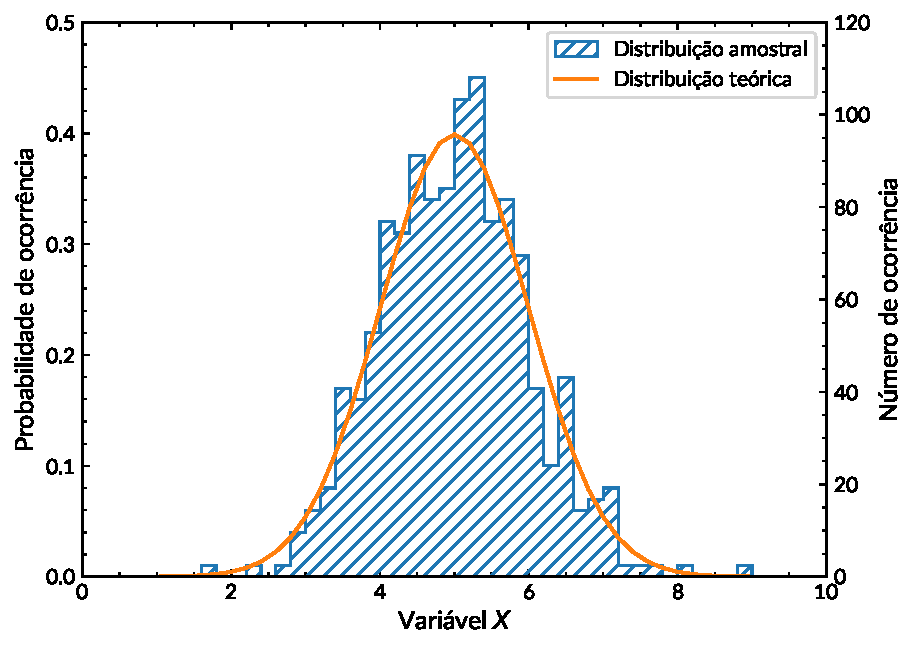
\includegraphics[width=0.7\linewidth]{Figuras/2-1.pdf}
	\caption{Distribuição amostral de uma variável aleatória $X$ a partir de 500 medições, obtida combinando as medições em intervalos de largura igual ($\Delta x = 0.2$). A forma da distribuição teórica depende da natureza do experimento e do número de medições, e neste exemplo é representada pela curva laranja.}
	\label{fig:2-1}
\end{SCfigure}

\section{Funções de Distribuição de Probabilidade}

É conveniente definir uma função que descreve a probabilidade de ocorrência da variável aleatória. Variáveis aleatórias discretas são descritas por uma \textbf{função de massa de probabilidade} (FMP) $f(x_i)$, onde $f(x_i)$ representa a probabilidade da variável ter um valor exato de $x_i$. Variáveis contínuas são descritas por uma \textbf{função de densidade de probabilidade} (FDP) $f(x)$, de modo que $f(x)\,dx$ é a probabilidade da variável estar no intervalo $[x, x + dx]$. Para simplicidade, a maioria das propriedades será ilustrada para variáveis contínuas, com a compreensão de que elas também se aplicam a variáveis discretas com modificações simples, como a substituição de uma integral por uma soma. Em princípio, também é possível ter variáveis aleatórias mais complexas que são parcialmente contínuas e parcialmente discretas. Um tratamento mais completo das variáveis aleatórias pode ser encontrado em qualquer livro-texto dedicado ao assunto, como os de \citet{ross2019introduction} ou \citet{siegrist2019random}. As funções de distribuição de probabilidade têm as seguintes propriedades-chave:

\begin{enumerate}[noitemsep]
\item Elas são normalizadas para 1. Para variáveis contínuas, isso significa que 
\begin{equation}
\int_{-\infty}^{\infty} f(x)\,dx = 1.
\end{equation}
Para variáveis definidas em um subconjunto dos números reais, por exemplo, apenas valores $x \geq 0$ ou em um intervalo finito, $f(x)$ é definido como zero fora do domínio de definição da função. Para variáveis discretas, a integral é substituída por uma soma sobre todos os valores que a variável pode assumir.

\item A distribuição de probabilidade nunca pode ser negativa, $f(x) \geq 0$. Isso é uma consequência do axioma de Kolmogorov, que requer que a probabilidade seja não negativa.

\item A \textbf{função de distribuição acumulada} (FDA) $F(x)$, ou simplesmente \textbf{função de distribuição}, 
\begin{equation}
F(x) = P(X \leq x) = \int_{-\infty}^{x} f(\tau)\, d\tau,
\end{equation}
representa a probabilidade de que a variável tenha um valor menor ou igual a $x$. $F(x)$ é uma função não decrescente de $x$ que começa em zero e tem seu maior valor de um. Uma função relacionada é a \textbf{função de sobrevivência} $S(x) = 1 - F(x)$, representando a probabilidade de $X > x$.
\end{enumerate}

\begin{exemplo}{}{}
A variável aleatória exponencial segue a FDP:
\begin{equation}
f(x) = \lambda e^{-\lambda x}, \quad x \geq 0,
\end{equation}
onde $\lambda$ é um parâmetro que deve ser positivo. Portanto, a FDP é $f(x) = 0$ para valores negativos da variável. A FDA é dada por:
\begin{equation}
F(x) = \int_{-\infty}^{x} \lambda e^{-\lambda \tau}\, d\tau =  \int_{-\infty}^{0} \lambda e^{-\lambda \tau}\, d\tau + \int_{0}^{x} \lambda e^{-\lambda \tau}\, d\tau  = 0 + \lambda\left(-\dfrac{1}{\lambda}e^{-\lambda \tau}\right)_0^{x} = 1 - e^{-\lambda x}.
\end{equation} 
Na \autoref{fig:2-2} estão representadas a FDP $f(x)$ e a FDA $F(x)$ para uma variável exponencial com $\lambda = 0.5$.
\begin{center}
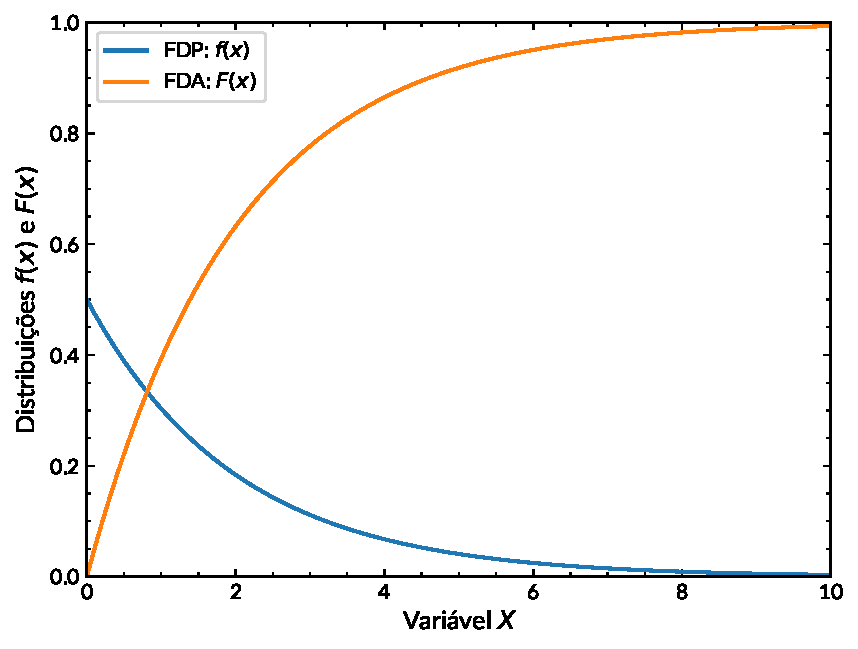
\includegraphics[width=0.65\linewidth]{Figuras/2-2.pdf}
\captionof{figure}{A função de distribuição $f(x)$ e a função de distribuição acumulada $F(x)$ para uma variável exponencial com $\lambda = 0.5$.}
\label{fig:2-2}
\end{center}
\end{exemplo}

\section{Expectância e Momentos de uma Função de Distribuição}

A função de densidade de probabilidade $f(x)$ ou a função de distribuição $F(x)$ fornece uma descrição completa da variável aleatória $X$. É conveniente encontrar algumas quantidades que descrevem os recursos mais importantes da distribuição. A \textbf{expectância} (ou \textbf{valor esperado}) de uma função determinística $g(x)$ da variável aleatória é definida por
\begin{equation}
\mathbb{E}[g(X)] = \int g(x) f(x)\, dx.
\end{equation}
O significado dessa expressão é que cada valor $g(x)$ é ponderado de acordo com a probabilidade de ocorrência de $x$, que é $f(x)$. A expectância é um operador linear, ou seja, satisfaz a propriedade
\begin{equation*}
\mathbb{E}[ag_1(x) + bg_2(x)] = a\,\mathbb{E}[g_1(x)] + b\,\mathbb{E}[g_2(x)]
\end{equation*}
devido à propriedade de linearidade da integral.

O \textbf{momento} de ordem $n$ é definido como
\begin{equation}
\mu_n = \mathbb{E}[X^n] =  \int x^n f(x)\, dx.
\end{equation}
Portanto, o momento $\mu_n$ é a expectância da função $g(x) = x^n$. É possível demonstrar, embora além do escopo deste livro, que o conhecimento dos momentos de todas as ordens é suficiente para determinar unicamente a função de distribuição \citep{wilks1947mathematical}. Este é um fato importante, pois transfere o problema de determinar a função de distribuição para o de determinar pelo menos alguns de seus momentos. Além disso, várias funções de distribuição têm apenas alguns momentos diferentes de zero, o que torna a tarefa ainda mais gerenciável.

Os momentos de uma distribuição são quantidades teóricas que podem ser calculadas a partir de  $f(x)$, sem qualquer referência a medidas. A seguir, são descritos dois dos momentos mais comumente utilizados, a média e a variância, e as quantidades amostrais que os aproximam, a média amostral e a variância amostral.

\subsection{A Média e a Média Amostral}

O momento de primeira ordem também é conhecido como \textbf{média} ou expectância da variável aleatória,
\begin{equation}\label{2.7}
	\mu = \mathbb{E}[X] = \int_{-\infty}^{\infty} x f(x)\, dx.
\end{equation}
A média $\mu$ é um número característico que representa um valor médio de $X$, obtido ponderando todos os valores possíveis da variável por sua função de distribuição. Portanto, a média é uma medida muito simples e conveniente da variável aleatória.

Para estimar a média da variável aleatória $X$, considere $N$ medidas $x_i$, com $i = 1, \ldots, N$. Cada medida $x_i$ pode ser considerada como uma amostra retirada aleatoriamente da distribuição populacional de $X$. A \textbf{média amostral} é definida como
\begin{equation}\label{2.8}
\overline{x} = \dfrac{1}{N} \sum_{i=1}^{N} x_i.
\end{equation}
É evidente que diferentes amostras de tamanho $N$ não resultarão no mesmo valor de $\overline{x}$, devido à aleatoriedade das medidas. Isso indica que $\overline{x}$ não é um número fixo, mas é ele próprio uma variável aleatória que deve ser escrita como
\begin{equation*}
	\overline{X} = \dfrac{1}{N} \sum_{i=1}^{N} X_i.
\end{equation*}
Esta nova equação é formalmente idêntica à \eqref{2.8} exceto pelo uso de letras maiúsculas, indicando que as quantidades são variáveis aleatórias, não apenas números. Portanto, é razoável perguntar se essa nova variável aleatória $\overline{X}$ tem a mesma expectância que a variável populacional $X$ em si. Essa pergunta pode ser facilmente respondida considerando que as variáveis $X_i$ são distribuídas de maneira idêntica da mesma forma que $X$, já que representam medidas aleatórias de $X$. A expectância de $\overline{X}$ é então:
\begin{equation*}
\mathbb{E}[\overline{X}] = \mathbb{E}\left[\dfrac{1}{N} \sum_{i=1}^{N} X_i\right] = \dfrac{1}{N}\sum_{i=1}^{N}\mathbb{E}[X_i] = \dfrac{N\mu}{N} = \mu.
\end{equation*}
A média amostral tem a mesma expectância que a variável populacional $X$, e portanto $\overline{X}$ é considerado um \textbf{estimador não tendencioso} de $X$. Esta é uma propriedade muito desejável, dado que a média amostral foi projetada exatamente com o propósito de estimar a variável populacional $X$ com suas medidas. Também se espera que, à medida que o número de medidas $N$ aumenta, a média amostral se aproxime cada vez mais da média populacional com maior precisão. Isso é mostrado na seção seguinte.

\subsection{A Lei dos Grandes Números}

A \textbf{lei dos grandes números} afirma que a média amostral converge para a média populacional conforme o tamanho da amostra aumenta, e é um dos teoremas fundamentais da probabilidade. Considere $N$ variáveis aleatórias $X_i$ que são identicamente distribuídas com $\mu$ sendo a média comum delas. A lei pode ser enunciada como:
\begin{equation}\label{2.9}
\lim\limits_{N \to \infty} \dfrac{X_1 + \cdots + X_N}{N} = \mu,
\end{equation}
Isso implica que a média amostral $X$ tende para a média $\mu$, que é um número determinístico e não uma variável aleatória. A \autoref{2.9} é uma afirmação muito forte porque mostra que, assintoticamente, a soma das variáveis aleatórias se torna uma constante igual à média amostral das $N$ variáveis, ou $N$ medidas. Embora não haja indicação sobre quão grande $N$ deve ser para alcançar esse objetivo, isso ainda é um resultado-chave para estabelecer o comportamento assintótico das variáveis aleatórias. É útil apontar que existem diferentes versões desta lei, de acordo com o método pelo qual essa convergência é estabelecida. Propriedades matemáticas desta lei e sua derivação podem ser encontradas em livros de teoria da probabilidade, como \citet{kolmogorov1950foundations,ross2019introduction}.

Essa lei também tem consequências importantes para funções de variáveis aleatórias. Dada uma função $g(x)$, seria conveniente estimar seu valor esperado $\mathbb{E}[g(X)]$ a partir das $N$ medidas das variáveis $X_i$. De acordo com a lei dos grandes números, é possível dizer que
\begin{equation}
	\lim\limits_{N \to \infty} \dfrac{g(X_1) + \cdots + g(X_N)}{N} = \mathbb{E}[g(X)].
\end{equation}
Essa expressão afirma que um grande número de medidas das variáveis $X_i$ pode ser usado para medir $\mathbb{E}[g(X)]$, contornando completamente a função de densidade de probabilidade da função $g(X)$. Essa propriedade será útil ao estudar a distribuição de funções de uma variável aleatória.

\subsection{A Variância e a Variância Amostral}

A \textbf{variância} é a expectância do quadrado da diferença entre $X$ e sua média,
\begin{equation}\label{2.11}
\text{Var}(X) = \mathbb{E}[(X - \mu)^2] = \int_{-\infty}^{+\infty} (x - \mu)^2 f(x)\,dx
\end{equation}
e geralmente é indicada como $\text{Var}(X) = \sigma^2$. A raiz quadrada da variância é referida como o \textbf{desvio padrão} $\sigma$, e é uma medida comum da diferença média de uma determinada medida $x_i$ da média da variável aleatória.

A principal razão para definir a média da diferença de uma medida de sua média em termos de um momento de segunda ordem é que a expectância da diferença $X - \mu$ é sempre zero:
\begin{equation*}
\mathbb{E}[X - \mu] = \mathbb{E}[X] - \mathbb{E}[\mu] = \mu - \mu = 0
\end{equation*}
Portanto, a diferença de uma variável aleatória não é comumente utilizada em estatísticas, uma vez que sua expectância é nula. Observe que as dimensões físicas dos momentos da ordem $n$ são aquelas da variável elevada à potência $n$. Por exemplo, se $X$ for medida em metros, a variância é medida em metros quadrados ($\text{m}^2$), enquanto o desvio padrão tem as mesmas dimensões que a variável e sua média.

Usando a propriedade linear da expectância, é simples mostrar que a seguinte propriedade se aplica:
\begin{equation}\label{2.12}
\text{Var}(X) = \mathbb{E}[(X - \mu)^2] = \mathbb{E}[X^2 - 2X\mu + \mu^2] = \mathbb{E}[X^2] - 2\mu^2 + \mu^2 = \mathbb{E}[X^2] - \mu^2.
\end{equation}
Essa relação é muito conveniente para calcular a variância a partir dos momentos de primeira e segunda ordem. Outra propriedade útil da variância, que decorre do fato de que a variância é um momento de segunda ordem, é
\begin{equation}\label{2.13}
\text{Var}(aX) = a^2 \cdot \text{Var}(X),
\end{equation}
onde $a$ é uma constante. O desvio e a variância são momentos calculados em relação à média, e são referidos como \textbf{momentos centrais}.

A \textbf{variância amostral} é definida como
\begin{equation}\label{2.14}
s^2 = \dfrac{1}{N -1} \sum_{i=1}^N (x_i - \overline{x})^2,
\end{equation}
uma nova variável aleatória que se destina a estimar a variância populacional $\sigma^2$ por meio de $N$ medições aleatórias. O fator $N - 1$, e não $N$, no denominador é necessário para garantir que a variância da amostra seja um estimador não tendencioso da variância populacional. Uma prova dessa propriedade é fornecida na \autoref{sec:2-6}.

\section{Covariância e Correlação entre Variáveis Aleatórias}

É comum medir mais de uma variável aleatória em um experimento dado. As variáveis frequentemente estão relacionadas entre si, e, portanto, é necessário definir uma medida de como uma variável afeta a medição das outras. Considere a medição tanto do comprimento de um lado de um quadrado quanto de sua área; é claro que as duas quantidades estão relacionadas de tal forma que a mudança de uma quantidade afeta a outra da mesma maneira, ou seja, uma mudança positiva no comprimento do lado resulta em uma mudança positiva na área. Nesse caso, o comprimento e a área serão ditos ter uma correlação positiva. Esta seção introduz conceitos-chave para estudar duas ou mais variáveis aleatórias simultaneamente.

\subsection{Distribuição de Probabilidade Conjunta e Momentos de Duas Variáveis Aleatórias}

Quando duas variáveis são medidas ao mesmo tempo, deseja-se saber a probabilidade de um par de medidas dado para as duas variáveis. Essa informação é fornecida pela \textbf{função de distribuição de probabilidade conjunta}, indicada como $h(x, y)$, onde $h(x, y)\,dxdy$ é a probabilidade de que as duas variáveis $X$ e $Y$ estejam em um intervalo bidimensional de tamanho $dxdy$ em torno do valor $(x, y)$. Essa função bidimensional pode ser representada experimentalmente por meio de sua distribuição amostral, da mesma forma que as distribuições unidimensionais.

Normalmente, é conveniente descrever o comportamento de uma variável de cada vez, mesmo que o experimento envolva mais de uma variável. O processo de considerar apenas uma variável de cada vez é chamado \textbf{marginalização}. A função de densidade de probabilidade marginal de $X$, ou seja, a função de distribuição de $X$ isoladamente, é obtida a partir da função de distribuição de probabilidade conjunta como:
\begin{equation}\label{2.15}
f_X(x) = \int_{-\infty}^{\infty} h(x,y) dy,
\end{equation}
com uma equação equivalente para a distribuição marginal de $Y$. A expectância de $X$ é definida como:
\begin{equation}
\mathbb{E}[X] = \int_{-\infty}^{\infty}\int_{-\infty}^{\infty} xh(x,y)\,dxdy = \mu_x,
\end{equation}
e similarmente a expectância de $Y$ é igual a:
\begin{equation*}
	\mathbb{E}[Y] = \int_{-\infty}^{\infty}\int_{-\infty}^{\infty} yh(x,y)\,dxdy = \mu_y.
\end{equation*}
A combinação dessas duas equações leva ao resultado:
\begin{equation*}
	\mathbb{E}[X + Y] = \int_{-\infty}^{\infty}\int_{-\infty}^{\infty} (x + y)h(x,y)\,dxdy = \mathbb{E}[X] + \mathbb{E}[Y],
\end{equation*}
o que significa que a expectância da soma de duas variáveis é igual à soma das expectâncias. Este é um resultado conveniente que se aplica a todas as variáveis aleatórias e pode ser generalizado para mais de duas variáveis, sendo geralmente referido como a propriedade linear da expectância. Em particular, é útil ressaltar que a propriedade linear se aplica independentemente da independência estatística entre as variáveis, que é introduzida mais adiante nesta seção.

A variância é definida de forma similar como:
\begin{equation}
\text{Var}(X) = \mathbb{E}[(X - \mu_x)^2] = \int_{-\infty}^{\infty}\int_{-\infty}^{\infty} (x - \mu_x)^2 h(x, y)\, dxdy = \sigma_x^2.
\end{equation}
Essas equações reconhecem o fato de que a outra variável, neste caso $Y$, é de fato parte do experimento, mas é considerada não interessante para o cálculo em questão. Portanto, a variável não interessante é integrada (ou somada) sobre, ponderada pela sua função de distribuição de probabilidade.

A \textbf{covariância} de duas variáveis aleatórias é definida como:
\begin{equation}\label{2.18}
\text{Cov}(X,Y) = \mathbb{E}[(X - \mu_x)(Y - \mu_y)] = \int_{-\infty}^{\infty}\int_{-\infty}^{\infty} (x - \mu_x)(y - \mu_y) h(x, y)\, dxdy
\end{equation}
e geralmente é representada como $\text{Cov}(X,Y) = \sigma_{xy}^2$. A covariância é a expectância do produto dos desvios das duas variáveis, e a ordem das duas variáveis é irrelevante, de modo que $\text{Cov}(X,Y) = \text{Cov}(Y,X)$. A covariância é positiva se, em média, um desvio positivo de $X$ for acompanhado por um desvio positivo de Y, ou se dois desvios negativos forem prováveis de ocorrer simultaneamente, de modo que o integrando seja uma quantidade positiva. Se, por outro lado, as duas variáveis tendem a ter desvios de sinais opostos, a covariância será negativa. A covariância, assim como a média e a variância, é uma quantidade populacional que pode ser calculada a partir da distribuição teórica das variáveis aleatórias. A covariância também pode ser calculada desenvolvendo o lado esquerdo da \autoref{2.18},
\begin{equation*}
	\text{Cov}(X,Y) = \mathbb{E}[(X - \mathbb{E}[X])(Y - \mathbb{E}[Y])] = \mathbb{E}[XY - X\mathbb{E}[Y] -\mathbb{E}[X]Y + \mathbb{E}[X]\mathbb{E}[Y]] = \mathbb{E}[XY] - \mathbb{E}[X]\mathbb{E}[Y],
\end{equation*}
e possui as seguintes propriedades lineares:
\begin{equation*}
\text{Cov}(X + a,Y + b) = \text{Cov}(X,Y) \qquad \text{e} \qquad \text{Cov}(aX + b,cY + d) = ac \cdot \text{Cov}(X,Y),
\end{equation*}
o que pode ser visto imediatamente a partir da definição de covariância e da propriedade linear da expectância. Outra propriedade útil é:
\begin{equation*}
	\text{Cov}(X + Z,Y) = \text{Cov}(X,Y) +\text{Cov}(Z,Y),
\end{equation*}
que pode ser comprovada expandindo as expectâncias, e pode ser generalizada para mais de duas variáveis.

A \textbf{covariância amostral} para uma coleção de $N$ pares de medidas é calculada como:
\begin{equation}\label{2.19}
	s_{xy}^2 = \dfrac{1}{N-1}\sum_{i=1}^N(x_i - \overline{x})(y_i - \overline{y}),
\end{equation}
usando uma equação similar à variância amostral. É possível mostrar que o denominador $(N - 1)$ é necessário para garantir que a covariância amostral seja um estimador não tendencioso da covariância populacional. Essa derivação é fornecida na \autoref{sec:2-6}.

A \textbf{correlação} é simplesmente uma versão normalizada da covariância:
\begin{equation}
\text{Cor}(X,Y) = \dfrac{\text{Cov}(X,Y)}{\sqrt{\text{Var}(X)\text{Var}(Y)}} = \dfrac{\sigma_{xy}^2}{\sigma_x\sigma_y},
\end{equation}
e pode ser indicada como $\text{Cor}(X,Y) = \rho$. A \textbf{desigualdade de Cauchy-Schwarz} é frequentemente declarada como:
\begin{equation}
\mathbb{E}[|XY|] \leq \sqrt{(\mathbb{E}[X^2]\mathbb{E}[Y^2])},
\end{equation}
e pode ser usada para mostrar que $-1 \leq \rho \leq 1$. Quando o coeficiente de correlação é zero, as duas variáveis são consideradas\textbf{ não correlacionadas}. O \textbf{coeficiente de correlação amostral} $r$ é calculado como:
\begin{equation}
r = \dfrac{s_{xy}^2}{s_{x}s_{y}} = \dfrac{\displaystyle\sum_{i=1}^N(x_i - \overline{x})(y_i - \overline{y})}{\sqrt{\displaystyle\sum_{i=1}^N(x_i - \overline{x})^2}\sqrt{\displaystyle\sum_{i=1}^N(y_i - \overline{y})^2}},
\end{equation}
onde $s_{xy}^2$ é a covariância amostral e $s_x^2$ e $s_y^2$ são as variâncias amostrais das duas variáveis, e os denominadores $(N - 1)$ tanto da covariância quanto das variâncias foram cancelados. A desigualdade de Cauchy-Schwarz pode ser usada novamente para mostrar que $-1 \leq r \leq 1$, assim como para a correlação populacional.

\subsection{Independência Estatística de Variáveis Aleatórias}

A independência entre eventos foi descrita e quantificada no \autoref{cap:1-1}, onde foi mostrado que dois eventos são independentes apenas quando a probabilidade de ambos os eventos ocorrerem (ou sua interseção) é o produto das probabilidades individuais. O conceito é estendido aqui para variáveis aleatórias, definindo duas variáveis aleatórias como independentes se e somente se a função de distribuição de probabilidade conjunta puder ser fatorada na seguinte forma:
\begin{equation}\label{2.23}
h(x, y) = f(x) \cdot g(y),
\end{equation}
onde as duas funções $f(x)$ e $g(y)$ se tornam as funções de distribuição de probabilidade das duas variáveis aleatórias. Quando duas variáveis são independentes, a função de distribuição de probabilidade marginal de cada variável, obtida por marginalização sobre a outra variável (ver \autoref{2.15}), é
\begin{equation}
	f_X(x) = \int_{-\infty}^{\infty} f(x) \cdot g(y) dy  = f(x),
\end{equation}
mostrando que $f(x)$ é de fato a função de distribuição marginal de $X$. Um resultado idêntico também é aplicável a $g(y)$.

É importante ressaltar que independência entre variáveis aleatórias e falta de correlação não são propriedades equivalentes. Independência, que é uma propriedade das funções de distribuição \eqref{2.23}, é uma propriedade muito mais forte do que a falta de correlação, que é baseada em uma afirmação que envolve apenas momentos. Pode ser provado que independência implica falta de correlação, mas não o contrário.

Podemos demostrar isso calculando a covariância de duas variáveis aleatórias independentes, com função de distribuição conjunta $h(x, y)$. A covariância é dada por:
\begin{equation*}
 \sigma_{xy} = \int_{-\infty}^{\infty} \int_{-\infty}^{\infty} (x - \mu_x)(y - \mu_y)h(x, y) \, dx \, dy = \int_{-\infty}^{\infty} (x - \mu_x) f(x) \, dx \int_{-\infty}^{\infty} (y - \mu_y) g(y) \, dy = 0,
\end{equation*}
onde cada integral se anula como a expectância da diferença de uma variável aleatória.

Como um contra-exemplo do fato de que variáveis dependentes podem ter um fator de correlação não nulo, considere o caso de uma variável aleatória $X$ com uma distribuição $f(x)$ que é simétrica em torno da origem, e outra variável $Y = X^2$. Elas não podem ser independentes pois estão relacionadas funcionalmente, mas será mostrado que a covariância delas é zero. A simetria em torno de zero implica $\mu_x = 0$. A média de $Y$ é $\mathbb{E}[Y] = \mathbb{E}[X^2] = \sigma_x^2$ já que a média de $X$ é nula (veja \autoref{2.12}). A partir disso, a covariância é dada por:
\begin{equation*}
\text{Cov}(X, Y) = \mathbb{E}[X(Y - \sigma_x^2)] = \mathbb{E}[X^3 - X \sigma_x^2] = \mathbb{E}[X^3] = 0 
\end{equation*}
devido à simetria de $f(x)$. Portanto, as duas variáveis $X$ e $X^2$ são não correlacionadas, mas não são independentes.

A variância da soma de duas ou mais variáveis independentes possui uma propriedade muito conveniente que é útil apresentar neste ponto. Considere a soma de $N$ variáveis independentes, $X = X_1 + \cdots + X_N$. A variância de $X$ possui a seguinte propriedade aditiva:
\begin{equation*}
\text{Var}(X) = \sum_{i=1}^{N} \text{Var}(X_i).
\end{equation*}
Para provar isso, considere a função de distribuição conjunta de $N$ variáveis independentes que pode ser fatorada de acordo com uma generalização simples da \autoref{2.23},
\begin{equation*}
h(x_1, \ldots, x_N) = f_1(x_1) \ldots f_N(x_N),
\end{equation*}
onde cada $f_i(x_i)$ representa a função de distribuição marginal da variável $X_i$, com média populacional $\mu_i$. A variância da soma pode ser escrita como
\begin{equation*}
\text{Var}(X) = \mathbb{E}[(X - \mu_X)^2] = \mathbb{E}[(X_1 + \cdots + X_N - (\mu_1 + \ldots + \mu_N))^2],
\end{equation*}
onde $\mu_X$ é a média da soma das variáveis, que é sempre igual à soma das médias. O quadrado pode ser expandido como
\begin{equation*}
\text{Var}(X) = \sum_{i=1}^{N} \mathbb{E}[(X_i - \mu_i)^2] + 2 \sum_{\substack{i > j}} \mathbb{E}[(X_i - \mu_i)(X_j - \mu_j)]
\end{equation*}
onde as expectâncias de todos os termos de produto cruzado na segunda soma são a covariância entre variáveis, que são todas nulas devido à independência delas. Isso leva à propriedade linear da variância, que se aplica apenas no caso de variáveis independentes.

\section{A Expectância da Variância Amostral e Covariância Amostral}\label{sec:2-6}

A variância amostral e a covariância amostral são valores que calculamos usando várias medições independentes de uma ou duas variáveis aleatórias. Assim como a média amostral, elas também são tratadas como variáveis aleatórias, o que significa que têm uma distribuição com seus momentos correspondentes. Por exemplo, para a média amostral, sua expectância foi calculada diretamente como $\mathbb{E}[x] = \mu$, onde $\mu$ é a média populacional da variável $X$. Isso mostra que a média amostral é um estimador imparcial da média populacional.

Considerações semelhantes precisam ser aplicadas à variância amostral e à covariância amostral, e assegurar se suas expectâncias concordam com as quantidades populacionais que foram projetadas para aproximar. As medidas que contribuem para essas variáveis amostrais são do tipo $x_i$, ou pares $(x_i, y_i)$, para $i = 1, \ldots, N$. As $N$ medidas são amostras independentes da variável $X$ ou do par de variáveis $X, Y$. Essa propriedade de independência entre as amostras é fundamental para entender a expectância das variáveis amostrais em questão. As medidas $x_i$ são ditas ser \textbf{variáveis independentes e identicamente distribuídas} (frequentemente abreviadas como IID), ou seja, amostras independentes da mesma distribuição populacional $f(x)$ com média populacional $\mu$. O mesmo se aplica ao caso bidimensional de pares $(x_i, y_i)$, que são amostras independentes de uma distribuição bidimensional populacional $h(x, y)$.

A seguinte derivação mostra que a expectância da variância amostral, conforme definida na \autoref{2.14}, é igual à variância populacional da variável $X$, e que a expectância da covariância amostral, conforme definida na \autoref{2.19}, é igual à covariância populacional. Essas propriedades mostram que a variância amostral e a covariância amostral são estimadores não enviesados das quantidades populacionais correspondentes. O fator de $N - 1$ no denominador deriva principalmente do fato de que as médias amostrais foram estimadas a partir dos dados, introduzindo uma fonte adicional de incerteza. Pode-se pensar nesta situação da seguinte maneira: as $N$ medidas, seja de uma única variável ou de um par de variáveis, são usadas primeiro para estimar a(s) média(s) amostral(is), reduzindo assim o número efetivo ou independente de medidas para $N - 1$.

Vamos então obter a expectância da variância amostral da seguinte maneira:
\begin{align*}
\mathbb{E}[s^2] &= \mathbb{E}\left[\dfrac{1}{N -1} \sum_{i=1}^N (x_i - \overline{x})^2,\right] \\
&= \left(\dfrac{1}{N -1}\right)\mathbb{E}\left[\sum_{i=1}^N (x_i - \mu + \mu - \overline{x})^2,\right] \\
&= \left(\dfrac{1}{N -1}\right)\mathbb{E}\left[\sum_{i=1}^N(x_i - \mu)^2 + \sum_{i=1}^N(\mu - \overline{x})^2 + 2(\mu - \overline{x})\sum_{i=1}^N(x_i - \mu)\right]
\end{align*}

O termo $\mathbb{E}[\textstyle\sum_{i=1}^{N} (\mu - \bar{x})^2]$ é $N$ vezes a variância da média amostral. Esta variância pode ser calculada observando que as $N$ medidas $x_i$ são, na verdade, variáveis aleatórias independentes com a mesma distribuição e mesma média $\mu$. A propriedade linear da variância, que só se aplica a variáveis independentes, leva a:
\begin{equation*}
\text{Var}(\overline{x}) = \dfrac{\text{Var}(x_1 + \cdots + x_n)}{N^2} = \frac{\sigma^2}{N},
\end{equation*}
onde $\sigma^2$ é a variância populacional de cada uma das variáveis $X_i$. O último termo na equação é $\textstyle\sum_{i=1}^{N} (x_i - \mu) = N (\overline{x} - \mu)$, portanto:
\begin{align*}
\mathbb{E}[s^2] &= \dfrac{1}{N -1}\left(\mathbb{E}\left[\sum_{i=1}^N(x_i - \mu)^2\right] + N\,\mathbb{E}\left[(\mu - \overline{x})^2\right] + 2N\,\mathbb{E}\left[(\mu - \overline{x})(\overline{x} - \mu)\right]\right) \\
&= \dfrac{1}{N -1}\left[N\sigma^2 + N\left(\dfrac{\sigma^2}{N}\right) - 2N\,\mathbb{E}\left[(\mu - \overline{x})^2\right]\right].
\end{align*}
Como $E[(\mu - \overline{x})^2]$ é novamente a variância da média amostral, a expectância da variância amostral é finalmente calculada como:
\begin{align*}
	\mathbb{E}[s^2] &= \dfrac{1}{N -1}\left[N\sigma^2 + N\left(\dfrac{\sigma^2}{N}\right) - 2N\left(\dfrac{\sigma^2}{N}\right)\right] = \sigma^2.
\end{align*}
Antes de calcular a expectância da covariância amostral, é necessário calcular a covariância entre as duas médias amostrais $\overline x$ e $\overline y$. De acordo com as propriedades da covariância:
\begin{align*}
 \text{Cov}(\overline x, \overline y) = \dfrac{1}{N^2}\left(\sum_{i=1}^{N}\text{Cov}(x_i,y_i) + 2 \sum_{i\neq j}^{N}\text{Cov}(x_i,y_i)\right).
\end{align*}
A independência entre pares de medidas significa que $\text{Cov}(x_i, y_j) = 0$ quando $i \neq j$. Além disso, como $\text{Cov}(x_i, y_i) = \sigma_{xy}^2$ é a covariância populacional, obtém-se o resultado:
\begin{align*}
\text{Cov}(\overline{x},\overline{y}) = \dfrac{\sigma_{xy}^2}{N}.
\end{align*}
A covariância amostral pode ser escrita como:
\begin{equation*}
s_{xy}^2 = \dfrac{1}{N-1}\sum_{i=1}^{N}(x_i - \overline{x})(y_i - \overline{y}) = \dfrac{1}{N-1} \left( \sum_{i=1}^{N} x_i y_i - N\overline{x}\,\overline{y}\right).
\end{equation*}
Uma vez que,
\begin{equation*}
\mathbb{E}[x_i y_i] = \sigma_{xy}^2 + \mu_x \mu_y \qquad \text{e} \qquad \mathbb{E}[\overline{x}\,\overline{y}] = \text{Cov}(\overline{x},\overline{y}) + \mathbb{E}[\overline{x}]\mathbb{E}[\overline{y}],
\end{equation*}
a expectância da covariância amostral é finalmente calculada como:
\begin{align*}
\mathbb{E}[s_{xy}^2] &= \left(\dfrac{1}{N-1}\right)\mathbb{E}\left[\sum_{i=1}^{N} x_i y_i - N\overline{x}\,\overline{y}\right] \\
&= \left(\dfrac{1}{N-1}\right)\left[N(\sigma_{xy}^2 + \mu_x \mu_y) - N\left(\text{Cov}(\overline{x},\overline{y}) + \mathbb{E}[\overline{x}]\mathbb{E}[\overline{y}]\right)\right] \\
&= \left(\dfrac{1}{N-1}\right)\left[N(\sigma_{xy}^2 + \mu_x \mu_y) - N\left(\dfrac{\sigma_{xy}^2}{N} + \mu_x \mu_y\right)\right] \\
&= \sigma_{xy}^2.
\end{align*}
Isso mostra que a covariância amostral é um estimador não enviesado da covariância populacional.

\section{Problemas}

\begin{enumerate}[label=\textbf{\arabic{chapter}.\arabic*.}]
	\item Considere a distribuição exponencial
	\begin{equation*}
	f(x) = \lambda e^{-\lambda x},
	\end{equation*}
	onde $\lambda > 0$ e $x \geq 0$. Mostre que a distribuição é devidamente normalizada e calcule a média e variância.
	
	\item Considere a média amostral como uma variável aleatória definida por
	\begin{equation*}
	\overline{x} = \dfrac{1}{N} \sum_{i=1}^{N} x_i,
	\end{equation*}
	onde $x_i$ são variáveis aleatórias independentes e idênticas com média $\mu$ e variância $\sigma^2$. Mostre que a variância de $\overline{x}$ é igual a $\sigma^2/N$.
	
	\item Nos experimentos pioneiros conduzidos por J.J. Thomson no final do século XIX, a intenção era medir a relação entre a massa e a carga de uma nova entidade subatômica, posteriormente denominada elétron. Este experimento não apenas introduziu um método revolucionário, mas também transformou nossa compreensão da física e das ciências naturais, ao demonstrar que essa nova partícula era consideravelmente mais leve do que o portador de carga conhecido na época, o próton. A abordagem experimental envolveu a deflexão de raios catódicos negativamente carregados por um campo magnético $H$ em um tubo de vácuo \citep{thomson1897xl}. Thomson procurou determinar a massa $m$ dessas partículas carregadas. Assim, o experimento foi baseado na medição de quantidades específicas: $W$, a energia cinética das partículas; $Q = Ne$, a carga elétrica total das partículas (onde $N$ é o número de partículas e $e$ é a carga elementar); e $I = HR$, onde $R$ é o raio de curvatura da trajetória das partículas no campo magnético $H$. Alguns dos dados experimentais coletados por Thomson são apresentados nas \autoref{tab:2-1} e \ref{tab:2-2}, onde ``gás'' se refere ao tipo de gás utilizado nos tubos de vácuo. Utilizando esses conjuntos de dados para os Tubos 1 e 2 separadamente, determine as médias amostrais e variâncias das variáveis aleatórias $W/Q$ e $I$, bem como a covariância e os coeficientes de correlação entre $W/Q$ e $I$.
	\begin{SCtable}[\sidecaptionrelwidth][!h]
		\centering
		\caption{Dados das medições de Thomson do Tubo 1.}
		\begin{tabular}{|l|l|l|l|l|}
			\hline
			Gás & $W/Q$ & $I$ & $m/e$ & $v$ \\
			\hline
			Ar & $4.6 \times 10^{11}$ & 230 & $0.57 \times 10^{-7}$ & $4 \times 10^{9}$ \\
			Ar & $1.8 \times 10^{12}$ & 350 & $0.34 \times 10^{-7}$ & $1 \times 10^{10}$ \\
			Ar & $6.1 \times 10^{11}$ & 230 & $0.43 \times 10^{-7}$ & $5.4 \times 10^{9}$ \\
			Ar & $2.5 \times 10^{12}$ & 400 & $0.32 \times 10^{-7}$ & $1.2 \times 10^{10}$ \\
			Ar & $5.5 \times 10^{11}$ & 230 & $0.48 \times 10^{-7}$ & $4.8 \times 10^{9}$ \\
			Ar & $1 \times 10^{12}$ & 285 & $0.4 \times 10^{-7}$ & $7 \times 10^{9}$ \\
			Ar & $1 \times 10^{12}$ & 285 & $0.4 \times 10^{-7}$ & $7 \times 10^{9}$ \\
			Hidrogênio & $6 \times 10^{12}$ & 205 & $0.35 \times 10^{-7}$ & $6 \times 10^{9}$ \\
			Hidrogênio & $2.1 \times 10^{12}$ & 460 & $0.5 \times 10^{-7}$ & $9.2 \times 10^{9}$ \\
			Ácido carbônico & $8.4 \times 10^{11}$ & 260 & $0.4 \times 10^{-7}$ & $7.5 \times 10^{9}$ \\
			Ácido carbônico & $1.47 \times 10^{12}$ & 340 & $0.4 \times 10^{-7}$ & $8.5 \times 10^{9}$ \\
			Ácido carbônico & $3.0 \times 10^{12}$ & 480 & $0.39 \times 10^{-7}$ & $1.3 \times 10^{10}$ \\
			\hline
		\end{tabular}
		\label{tab:2-1}
	\end{SCtable}
	
	\begin{SCtable}[\sidecaptionrelwidth][!h]
		\centering
		\caption{Dados das medições de Thomson do Tubo 2.}
		\begin{tabular}{|l|l|l|l|l|}
			\hline
			Gás & $W/Q$ & $I$ & $m/e$ & $v$ \\
			\hline
			Ar & $2.8 \times 10^{11}$ & 175 & $0.53 \times 10^{-7}$ & $3.3 \times 10^{9}$ \\
			Ar & $2.8 \times 10^{11}$ & 175 & $0.47 \times 10^{-7}$ & $4.1 \times 10^{9}$ \\
			Ar & $3.5 \times 10^{11}$ & 181 & $0.47 \times 10^{-7}$ & $3.8 \times 10^{9}$ \\
			Hidrogênio & $2.8 \times 10^{11}$ & 175 & $0.53 \times 10^{-7}$ & $3.3 \times 10^{9}$ \\
			Ar & $2.5 \times 10^{11}$ & 160 & $0.51 \times 10^{-7}$ & $3.1 \times 10^{9}$ \\
			Ácido carbônico & $2.0 \times 10^{11}$ & 148 & $0.54 \times 10^{-7}$ & $2.5 \times 10^{9}$ \\
			Ar & $1.8 \times 10^{11}$ & 151 & $0.63 \times 10^{-7}$ & $2.3 \times 10^{9}$ \\
			Hidrogênio & $2.8 \times 10^{11}$ & 175 & $0.53 \times 10^{-7}$ & $3.3 \times 10^{9}$ \\
			Hidrogênio & $4.4 \times 10^{11}$ & 201 & $0.46 \times 10^{-7}$ & $4.4 \times 10^{9}$ \\
			Ar & $2.5 \times 10^{11}$ & 176 & $0.61 \times 10^{-7}$ & $2.8 \times 10^{9}$ \\
			Ar & $4.2 \times 10^{11}$ & 200 & $0.48 \times 10^{-7}$ & $4.1 \times 10^{9}$ \\
			\hline
		\end{tabular}
		\label{tab:2-2}
	\end{SCtable}
	
	\item Ainda usando o experimento de J.J. Thomson, verifique a afirmação de que
	\begin{quote}
	\textit{O valor de $m/e$ é independente da natureza do gás.}
	\end{quote}
	Você pode fazer isso calculando a média amostral e o desvio padrão para as medições em cada gás (ar, hidrogênio e ácido carbônico), e então testando se as três medições concordam entre si dentro de seus desvios padrão.
	
	\item Calcule a covariância amostral e o coeficiente de correlação para o seguinte conjunto de dados: $(0, 2), (2, 5), (1, 4), (3, 1)$.
\end{enumerate}




\chapter*{Resolução dos Problemas}
\addcontentsline{toc}{chapter}{Resolução dos Problemas}

\section*{Capítulo 1}
\addcontentsline{toc}{section}{Capítulo 1}

\begin{enumerate}[label=\textbf{1.\arabic*.}]
\item \label{r1.1} Considere o lançamento de quatro moedas iguais em sequência, onde $\text{Cara}$ é representada por $\text{C}$ e $\text{Coroa}$ por $\text{K}$. O espaço amostral para esse experimento é:
\begin{align*}
	\Omega &= \{\text{CCCC}, \text{CCCK}, \text{CCKC}, \text{CKCC}, \text{KCCC}, \text{CCKK}, \text{CKCK}, \text{KCKC}, \\ 
	&\qquad\text{CKKC}, \text{KKCC}, \text{KCCK}, \text{KKKC}, \text{KKCK}, \text{KCKK}, \text{CKKK}, \text{KKKK}\}.
\end{align*}
Assumindo que as moedas são imparciais, cada evento tem a mesma probabilidade de $\sfrac{1}{16}$. A probabilidade de obter duas caras e duas coroas, ou seja, os eventos $\{ \text{CCKK}, \text{CKCK}, \text{KCKC}, \text{CKKC}, \text{KKCC}, \text{KCCK}\}$ é $\sfrac{6}{16} = \sfrac{3}{8}$.

\item Considere os eventos:
\begin{align*}
	A = \{ \text{primeiro lançamento mostra número ímpar} \}, \quad \text{e} \quad
	B = \{ \text{soma dos dois dados é 9} \}.
\end{align*}
O evento $A$ ocorre nos resultados $1, 3,$ e $5$ (como cada evento tem uma probabilidade $\sfrac{1}{6}$), assim $P(A) = \sfrac{1}{2}$. Para calcular $P(B)$, os pares que somam 9 são $(3,6), (4,5), (5,4),$ e $(6,3)$, portanto $P(B) = \sfrac{4}{36} = \sfrac{1}{9}$. A probabilidade da união de $A$ e $B$ deve excluir a interseção deles para evitar duplicações, que são os lançamentos $(3,6)$ e $(5,4)$, onde $P(A \cap B) = \sfrac{1}{8}$. Portanto, considerando o terceiro axioma de Kolmogorov generalizado (\autoref{1.5}), temos que a probabilidade do primeiro lançamento mostra um número ímpar ou a soma dos dois dados é 9 é
\begin{equation*}
P(A \cup B) = P(A) + P(B) - P(A \cap B) = \dfrac{1}{2} + \dfrac{1}{9} - \dfrac{1}{18} = \dfrac{5}{18}.
\end{equation*}

\item Considere os eventos:
\begin{align*}
	A = \{ \text{obter número par} \}, \quad \text{e} \quad
	B = \{ \text{obter número maior que 4} \}.
\end{align*}
O evento $A$ ocorre nos resultados $2, 4,$ e $6$, assim $P(A) = \sfrac{3}{6}  = \sfrac{1}{2}$. Para calcular $P(B)$, os resultados maiores que 4 são $5$ e $6$, portanto $P(B) = \sfrac{2}{6} = \sfrac{1}{3}$. A interseção de $A$ e $B$ ocorre apenas em $6$, assim $P(A \cap B) = \sfrac{1}{6}$. Assim, pelo terceiro axioma de Kolmogorov generalizado (\autoref{1.5}), temos:
\begin{equation*}
P(A \cup B) = P(A) + P(B) - P(A \cap B) = \dfrac{1}{2} + \dfrac{1}{3} - \dfrac{1}{6} = \dfrac{2}{3}.
\end{equation*}

\item Considere os eventos:
\begin{align*}
	A = \{ \text{soma dos dois lançamentos é 8} \}, \quad \text{e} \quad
	B = \{ \text{o primeiro lançamento mostra 5} \}.
\end{align*}
O evento $A$ ocorre para as seguintes combinações de resultados: $(2,6), (3,5), (4,4), (5,3), (6,2)$ e portanto $P(A) = \sfrac{5}{36}$. O evento $B$ tem uma probabilidade $P(B) = \sfrac{1}{6}$. O evento $A \cap B$ tem probabilidade $P(A \cap B) = \sfrac{1}{36}$ (situação em que ambos os eventos ocorrem, no caso, quando ocorrer o resultado $(5,3)$). Como
\begin{equation*}
P(A) \cdot P(B) = \dfrac{5}{36} \cdot \dfrac{1}{6} = \dfrac{5}{1296} \neq P(A \cap B) = \dfrac{1}{36},
\end{equation*}
os dois eventos não são estatisticamente independentes.

\item Considere os seguintes eventos:
\begin{align*}
	A = \{ \text{o primeiro lançamento é par} \}, \quad \text{e} \quad
	B = \{ \text{o segundo lançamento é par} \}.
\end{align*}
O evento $A$ ocorre para $2,4,6$ (bem como o evento $B$) e portanto $P(A) = \sfrac{3}{6} = \sfrac{1}{2}$ (analogamente, $P(B) = \sfrac{1}{2}$). O evento $A \cap B$, que ocorre para as seguintes combinações de resultados: $(2,2), (2,4), (2,6), (4,2), (4,4), (4,6), (6,6), (6,2), (6,4)$, tem probabilidade $P(A \cap B) = \sfrac{9}{36} = \sfrac{1}{4}$. Como
\begin{equation*}
	P(A) \cdot P(B) = \dfrac{1}{2} \cdot \dfrac{1}{2} = \dfrac{1}{4} = P(A \cap B) = \dfrac{1}{4},
\end{equation*}
os dois eventos são estatisticamente independentes.

\item A probabilidade de retirar uma bola vermelha é $p = \sfrac{3}{5}$, já que 3 das 5 bolas são vermelhas. (a) Os sorteios consecutivos são independentes e, portanto, a probabilidade de duas bolas vermelhas consecutivas é $p = \sfrac{3}{5} \cdot \sfrac{3}{5} = \sfrac{9}{25}$, já que os sorteios são feitos com reposição. (b) A condição de que o primeiro sorteio foi uma bola vermelha é irrelevante para o resultado do segundo sorteio, e portanto a probabilidade é apenas $p = \sfrac{3}{5}$. A solução também pode ser obtida usando a definição de probabilidade condicional (\autoref{1.6}) e a definição de independência estatística (\autoref{1.8}),
\begin{equation*}
P(B|A) = \dfrac{P(A \cap B)}{P(A)} = \dfrac{P(A)\cdot P(B)}{P(A)} = P(B) = \dfrac{3}{5}
\end{equation*}
onde $A$ é o evento de uma bola vermelha no primeiro sorteio e $B$ é o evento de uma bola vermelha no segundo sorteio.

\item A probabilidade do dado der $1$ (evento $A$) é $P(A) = \sfrac{1}{6}$, e a probabilidade da soma ser $5$ (evento $B$) é $P(B) = \sfrac{4}{36}$, já que as sequências que resultam em uma soma de $5$ são apenas quatro: $(2,3), (3,2), (4,1), (1,4)$. (a) A probabilidade de $A$ dado $B$ é,
\begin{equation*}
P(A|B) = \dfrac{P(A \cap B)}{P(B)} = \dfrac{\sfrac{1}{36}}{\sfrac{4}{36}} = \dfrac{1}{4},
\end{equation*}
já que $P(A \cap B) = \sfrac{1}{36}$ representa a probabilidade da única combinação $(1, 4)$ ocorrer. (b) A probabilidade de $B$ dado $A$ é,
\begin{equation*}
	P(B|A) = \dfrac{P(B \cap A)}{P(A)} = \dfrac{\sfrac{1}{36}}{\sfrac{1}{6}} = \dfrac{1}{6},
\end{equation*}
(c) A probabilidade do primeiro lançamento ser $1$ e a soma ser $5$ é simplesmente,
\begin{equation*}
P(A \cap B) = P(A|B)\cdot P(B) = \dfrac{1}{4} \times \dfrac{4}{36} = \dfrac{1}{36}.
\end{equation*}
(d) Usando a \autoref{1.11}, podemos mostrar que,
\begin{equation*}
P(A | B) = \dfrac{P(B | A)P(A)}{P(B)} = \dfrac{\sfrac{1}{6} \times \sfrac{1}{6}}{\sfrac{4}{36}} = \dfrac{1}{4}.
\end{equation*}
o teorema de Bayes é verificado.

\item (a) Uma sequência específica tem uma probabilidade de $P(A) = (\sfrac{1}{2})^4 = \sfrac{1}{16}$, já que os quatro lançamentos são independentes, e cada um tem uma probabilidade de \sfrac{1}{2} de cara. (b) Precisamos contar o número de sequências que têm 2 moedas caindo cara (evento $B$). Usando o resultado do Problema \ref{r1.1}, vemos que existem 6 dessas sequências, e portanto a probabilidade é $P(B) = \sfrac{6}{16} = \sfrac{3}{8}$ por contagem direta. O evento $B$ inclui $A$, portanto a probabilidade da interseção é $P(A \cap B) = \sfrac{1}{16}$. A probabilidade de uma sequência cara-coroa-cara-coroa dado que duas moedas caíram com a face para cima é
\begin{equation*}
P(A|B) = \dfrac{P(A \cap B)}{P(B)} = \dfrac{\sfrac{1}{16}}{\sfrac{3}{8}} = \dfrac{1}{6}
\end{equation*}
(c) Para isso, podemos usar o teorema de Bayes (\autoref{1.11}), 
\begin{equation*}
P(B | A) = \dfrac{P(A | B)P(B)}{P(A)} = \dfrac{\sfrac{1}{6}\times\sfrac{3}{8}}{\sfrac{1}{16}} = 1. 
\end{equation*}
O conhecimento da sequência cara-coroa-cara-coroa de fato implica a certeza de que 2 moedas caíram cara.
\end{enumerate}


\addcontentsline{toc}{chapter}{Referências Bibliográficas}
\bibliographystyle{plainnat-reversed}
\bibliography{referencias}
\end{document}